\documentclass[]{article}
\usepackage{hyperref}
\usepackage{multirow}
\usepackage{float}
\usepackage{textcomp}
\usepackage{graphicx}
\usepackage{float}
% Title Page
\title{Low-Comotovation: System Design Document}
\author{Michael Ghaben}
\date{}

\begin{document}

\maketitle
\tableofcontents
\titlepage

\subsection{Versioning \& Authorship}
Version 0.1
\newline
Low-Comotovation \textcopyright

\raggedright
Software Design Specification: Low-Comotovation \\
Status: Preliminary Release: Software Design Review

\subsection{References}
During the development of this document, IEEE 1016 was utilized.

\subsection{Purpose}
This document will specify the architecture and design of the Low-Comotovation train system. It shall discuss the structural and design and considerations of the train system and the accompanying subsystems of the train system. It shall also detail design considerations in vital subsystems.

\subsection{Stakeholders \& Concerns}
The stakeholders of this document are anticipated to be the following:
\begin{itemize}
	\item Future Design Teams: Future design teams are anticiapted to utilize this document to guide their usage of the track controller system
	\item Pittsburgh Rail Company: The rail company utlizing the Software Design Specification (SDS) to guide the development of physical systems associated with the software
\end{itemize}

Future design teams associated with the continued development beneift from increased documentation of the original system by allowing for more efficient software design procedures in future revision by potentially unrelated developers.

The benefits to the Pittsburgh Rail Company from  a detailed software design specification are twofold. First, a detailed SDD provides developers of railway hardware the information required to produced a paired system. Second, a documented SDD allows the Pittsburgh Rail Company to evaluate the designs ability to meet specifications for vitality.

\section{Introduction}
To ensure safe, predictable, and reliable operation of the system, there are three primary considerations:
\begin{enumerate}
	\item \emph{Vitality:} Vitality of a system within this document referse to a safety-critical system.
	\item \emph{Testability:} Any system implemented must be easily tested to ensure reliability
	\item \emph{Modularity:} Any system designed must reuse code wherever possible
\end{enumerate}

\section{System Design Use Cases}
In this section, we detail the use cases of each subsystem. The use case of each subsystem is accompanied by brief descriptions of the use cases.

\subsection{Track Model}
In this subsection, the use cases of the train model are provided.

\begin{figure}[H]
	\centering
	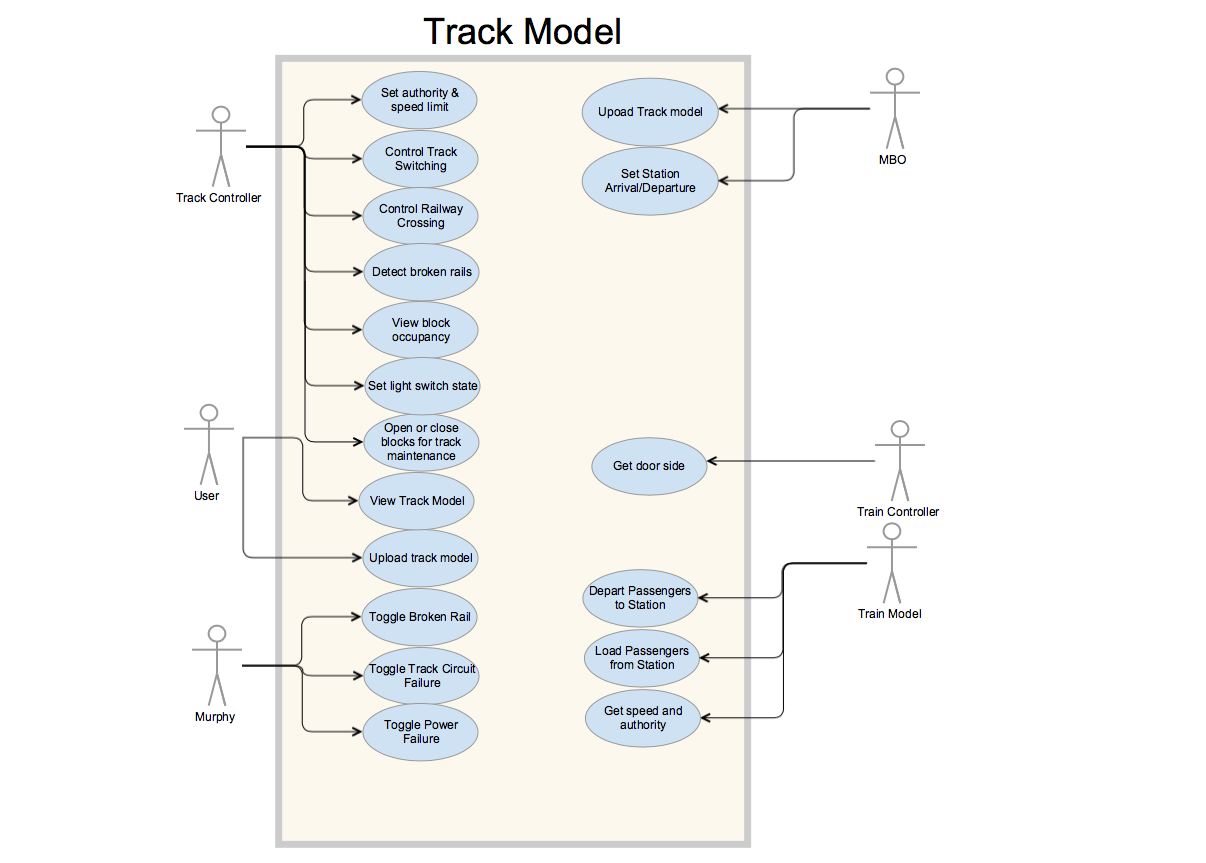
\includegraphics[scale=.3]{trackmodelusecase.png}
	\caption{Track model use case diagram}
\end{figure}
   \begin{table}[H]
   	\centering
   	\caption{Set Speed and Authority}
   	\begin{tabular}{|l|l|}
   		\hline
   		Actors & \parbox[t]{10cm}{Track Controller} \\ \hline
   		Description & \parbox[t]{10cm}{The track controller shall be capable of setting a speed and authority via the track circuit modeled by the track model} \\ \hline
   		Data &  \parbox[t]{10cm}{Speed and authority for the trains} \\ \hline
   		Stimulus &  \parbox[t]{10cm}{None. The speed and authority are set externally } \\ \hline
   		Response & \parbox[t]{10cm}{The track model possesses the attributes set.}\\ \hline
   		Comments & \parbox[t]{10cm}{ The track model only exists as a passthrough for this information }  \\ \hline
   	\end{tabular}
   \end{table}
   
   \begin{table}[H]
   	\centering
   	\caption{Set Switch State}
   	\begin{tabular}{|l|l|}
   		\hline
   		Actors & \parbox[t]{10cm}{Track Controller} \\ \hline
   		Description & \parbox[t]{10cm}{The track controller shall be capable of setting the switch of a given state} \\ \hline
   		Data &  \parbox[t]{10cm}{A boolean statement for the state of a switch} \\ \hline
   		Stimulus &  \parbox[t]{10cm}{The Track Controller signal } \\ \hline
   		Response & \parbox[t]{10cm}{Setting the state of the switch}\\ \hline
   		Comments & \parbox[t]{10cm}{ These are set simultaneously with no delays }  \\ \hline
   	\end{tabular}
   \end{table}
   
   \begin{table}[H]
   	\centering
   	\caption{Control Railyway Crossing}
   	\begin{tabular}{|l|l|}
   		\hline
   		\hline
   		Actors & \parbox[t]{10cm}{Track Controller} \\ \hline
   		Description & \parbox[t]{10cm}{The track controller shall be capable of setting the railway crossing to a given state} \\ \hline
   		Data &  \parbox[t]{10cm}{A boolean statement for the state of a railway crossing} \\ \hline
   		Stimulus &  \parbox[t]{10cm}{The Track Controller boolean signal } \\ \hline
   		Response & \parbox[t]{10cm}{Setting the state of the railway crossing}\\ \hline
   		Comments & \parbox[t]{10cm}{ These are set simultaneously with no delays }  \\ \hline
   	\end{tabular}
   \end{table}
   
   \begin{table}[H]
   	\centering
   	\caption{Detect Broken Rails}
   	\begin{tabular}{|l|l|}
   		\hline
   		Actors & \parbox[t]{10cm}{Track Controller} \\ \hline
   		Description & \parbox[t]{10cm}{The track controller shall be capable of detecting broken rails} \\ \hline
   		Data &  \parbox[t]{10cm}{A boolean statement for the state of a block} \\ \hline
   		Stimulus &  \parbox[t]{10cm}{A track controller query } \\ \hline
   		Response & \parbox[t]{10cm}{A return of the boolean broken state of the blocks on a track }\\ \hline
   		Comments & \parbox[t]{10cm}{ The track controller calls the track model in this case}  \\ \hline
   	\end{tabular}
   \end{table}
   
   \begin{table}[H]
   	\centering
   	\caption{View Block Occupancy}
   	\begin{tabular}{|l|l|}
   		\hline
   		Actors & \parbox[t]{10cm}{Track Controller} \\ \hline
   		Description & \parbox[t]{10cm}{The track controller shall be capable of viewing block occupancy} \\ \hline
   		Data &  \parbox[t]{10cm}{A boolean statement for the occupancy of the block} \\ \hline
   		Stimulus &  \parbox[t]{10cm}{A track controller query } \\ \hline
   		Response & \parbox[t]{10cm}{A return of the boolean occupied state of the blocks on a trackl }\\ \hline
   		Comments & \parbox[t]{10cm}{ The track controller calls the track model in this case}  \\ \hline
   	\end{tabular}
   \end{table}
   
   \begin{table}[H]
   	\centering
   	\caption{Set Light Switch State}
   	\begin{tabular}{|l|l|}
   		\hline
   		Actors & \parbox[t]{10cm}{Track Controller} \\ \hline
   		Description & \parbox[t]{10cm}{The track controller shall be capable of setting the light states} \\ \hline
   		Data &  \parbox[t]{10cm}{A boolean statement for the next light switch state} \\ \hline
   		Stimulus &  \parbox[t]{10cm}{A track controller function call } \\ \hline
   		Response & \parbox[t]{10cm}{A setting of the light switch state to that set by the track controller }\\ \hline
   		Comments & \parbox[t]{10cm}{ }  \\ \hline
   	\end{tabular}
   \end{table}
   
   \begin{table}[H]
   	\centering
   	\caption{Set Light Switch State}
   	\begin{tabular}{|l|l|}
   		\hline
   		Actors & \parbox[t]{10cm}{Track Controller} \\ \hline
   		Description & \parbox[t]{10cm}{The track controller shall be opening or closing a given block for maintenance} \\ \hline
   		Data &  \parbox[t]{10cm}{A boolean statement for if a given block is open or closed due to maintenance} \\ \hline
   		Stimulus &  \parbox[t]{10cm}{A track controller function call with a boolean variable } \\ \hline
   		Response & \parbox[t]{10cm}{A setting of the blocks open state }\\ \hline
   		Comments & \parbox[t]{10cm}{ This block will not be considered "open" for planning purposes in new path. This is reflected in the nextBlock functionality}  \\ \hline
   	\end{tabular}
   \end{table}
   
   \begin{table}[H]
   	\centering
   	\caption{Upoad Track Model}
   	\begin{tabular}{|l|l|}
   		\hline
   		Actors & \parbox[t]{10cm}{User} \\ \hline
   		Description & \parbox[t]{10cm}{The user shall be capable of uploading track models to the track model} \\ \hline
   		Data &  \parbox[t]{10cm}{The track model given in a .csv form. This may be provided by Excel "save as" function or similar.} \\ \hline
   		Stimulus &  \parbox[t]{10cm}{None} \\ \hline
   		Response & \parbox[t]{10cm}{The user loads the files in }\\ \hline
   		Comments & \parbox[t]{10cm}{This will require multiple csv files in practice }  \\ \hline
   	\end{tabular}
   \end{table}
   \begin{table}[H]
   	\centering
   	\caption{Set Light Switch State}
   	\begin{tabular}{|l|l|}
   		\hline
   		Actors & \parbox[t]{10cm}{Track Controller} \\ \hline
   		Description & \parbox[t]{10cm}{The track controller shall be capable of setting the light states} \\ \hline
   		Data &  \parbox[t]{10cm}{A boolean statement for the next light switch state} \\ \hline
   		Stimulus &  \parbox[t]{10cm}{A track controller function call } \\ \hline
   		Response & \parbox[t]{10cm}{A setting of the light switch state to that set by the track controller }\\ \hline
   		Comments & \parbox[t]{10cm}{ }  \\ \hline
   	\end{tabular}
   \end{table}
   
   \begin{table}[H]
   	\centering
   	\caption{Toggle Broken Rail}
   	\begin{tabular}{|l|l|}
   		\hline
   		Actors & \parbox[t]{10cm}{Murphy} \\ \hline
   		Description & \parbox[t]{10cm}{A test environment shall be provided to toggle the rail broken state for testing} \\ \hline
   		Data &  \parbox[t]{10cm}{A boolean statement to set the rail to} \\ \hline
   		Stimulus &  \parbox[t]{10cm}{External user testing stimulus} \\ \hline
   		Response & \parbox[t]{10cm}{Setting a given block to broken or fixed}\\ \hline
   		Comments & \parbox[t]{10cm}{ This should be considered for test purposes of other modules}  \\ \hline
   	\end{tabular}
   \end{table}
   
   \begin{table}[H]
   	\centering
   	\caption{Toggle Track Circuit Failure}
   	\begin{tabular}{|l|l|}
   		\hline
   		Actors & \parbox[t]{10cm}{Murphy} \\ \hline
   		Description & \parbox[t]{10cm}{A test environment shall be provided to toggle the circuit failure state for testing} \\ \hline
   		Data &  \parbox[t]{10cm}{A boolean statement to set the track circuit functionality} \\ \hline
   		Stimulus &  \parbox[t]{10cm}{External user testing stimulus} \\ \hline
   		Response & \parbox[t]{10cm}{Setting the track circuit to broken or functional}\\ \hline
   		Comments & \parbox[t]{10cm}{ This should be considered for test purposes of other modules}  \\ \hline
   	\end{tabular}
   \end{table}
   
   \begin{table}[H]
   	\centering
   	\caption{Toggle Power Failure}
   	\begin{tabular}{|l|l|}
   		\hline
   		Actors & \parbox[t]{10cm}{Murphy} \\ \hline
   		Description & \parbox[t]{10cm}{A test environment shall be provided to toggle the power failure state for testing} \\ \hline
   		Data &  \parbox[t]{10cm}{A boolean statement to set the power failure state of a rail to} \\ \hline
   		Stimulus &  \parbox[t]{10cm}{External user testing stimulus} \\ \hline
   		Response & \parbox[t]{10cm}{Setting a broken or fixed power state to}\\ \hline
   		Comments & \parbox[t]{10cm}{ This should be considered for test purposes of other modules}  \\ \hline
   	\end{tabular}
   \end{table}
   
   \begin{table}[H]
   	\centering
   	\caption{Upload Track Module}
   	\begin{tabular}{|l|l|}
   		\hline
   		Actors & \parbox[t]{10cm}{MBO} \\ \hline
   		Description & \parbox[t]{10cm}{Upload a track model to the track module} \\ \hline
   		Data &  \parbox[t]{10cm}{identical to the user inputs} \\ \hline
   		Stimulus &  \parbox[t]{10cm}{Initialization of a program} \\ \hline
   		Response & \parbox[t]{10cm}{The reading of the excel file}\\ \hline
   		Comments & \parbox[t]{10cm}{Functionally equivalent to the read track info for the user}  \\ \hline
   	\end{tabular}
   \end{table}
	 \begin{table}[H]
	 	\centering
	 	\caption{Set Station Arrival/Departure}
	 	\begin{tabular}{|l|l|}
	 		\hline
	 		Actors & \parbox[t]{10cm}{MBO} \\ \hline
	 		Description & \parbox[t]{10cm}{Set station arrival and departure time} \\ \hline
	 		Data &  \parbox[t]{10cm}{Receives the expected arrival and departure time from the MBO and displays them at a station} \\ \hline
	 		Stimulus &  \parbox[t]{10cm}{The MBO setting an arrival or departure at a given station} \\ \hline
	 		Response & \parbox[t]{10cm}{Setting an arrival or departure at a given station}\\ \hline
	 		Comments & \parbox[t]{10cm}{Set and called by the MBO}  \\ \hline
	 	\end{tabular}
	 \end{table}
	  \begin{table}[H]
	  	\centering
	  	\caption{Get Door Side}
	  	\begin{tabular}{|l|l|}
	  		\hline
	  		Actors & \parbox[t]{10cm}{Train Controller} \\ \hline
	  		Description & \parbox[t]{10cm}{Get the side of the door for arrival at a station given the visible beacon} \\ \hline
	  		Data &  \parbox[t]{10cm}{Returns the side of the door to open for a given train} \\ \hline
	  		Stimulus &  \parbox[t]{10cm}{Query with a station given a beacon} \\ \hline
	  		Response & \parbox[t]{10cm}{Side of the train to open the door on}\\ \hline
	  		Comments & \parbox[t]{10cm}{Set and called by the Train Conroller}  \\ \hline
	  	\end{tabular}
	  \end{table}
	  
	  \begin{table}[H]
	  	\centering
	  	\caption{Depart Passengers to Station}
	  	\begin{tabular}{|l|l|}
	  		\hline
	  		Actors & \parbox[t]{10cm}{Train Model} \\ \hline
		   	Description & \parbox[t]{10cm}{Depart passengers from a train to a station} \\ \hline
	  		Data &  \parbox[t]{10cm}{Number of passengers to depart} \\ \hline
	  		Stimulus &  \parbox[t]{10cm}{Train model calling the station of the track model} \\ \hline
	  		Response & \parbox[t]{10cm}{Add the people to the station loitering group}\\ \hline
	  		Comments & \parbox[t]{10cm}{Set and called by the Train Model}  \\ \hline
	  	\end{tabular}
	  \end{table}
	  
	  \begin{table}[H]
	  	\centering
	  	\caption{Get speed and authority from a given block}
	  	\begin{tabular}{|l|l|}
	  		\hline
	  		Actors & \parbox[t]{10cm}{Train Model} \\ \hline
	  		Description & \parbox[t]{10cm}{Calls a given block} \\ \hline
	  		Data &  \parbox[t]{10cm}{Number of passengers to depart} \\ \hline
	  		Stimulus &  \parbox[t]{10cm}{Train model calling the station of the track model} \\ \hline
	  		Response & \parbox[t]{10cm}{Return speed and authority at a given block}\\ \hline
	  		Comments & \parbox[t]{10cm}{Set and called by the Train Model}  \\ \hline
	  	\end{tabular}
	  \end{table}
	  
	  \begin{table}[H]
	  	\centering
	  	\caption{Load Passengers From Station}
	  	\begin{tabular}{|l|l|}
	  		\hline
	  		Actors & \parbox[t]{10cm}{Train Controller} \\ \hline
	  		Description & \parbox[t]{10cm}{Load passengers to a track model from a station} \\ \hline
	  		Data &  \parbox[t]{10cm}{Maximum number of passengers to load a train to capacity} \\ \hline
	  		Stimulus &  \parbox[t]{10cm}{Train model queryiing the track model} \\ \hline
	  		Response & \parbox[t]{10cm}{Number of people to add to the train}\\ \hline
	  		Comments & \parbox[t]{10cm}{Set and called by the Train Conroller}  \\ \hline
	  	\end{tabular}
	  \end{table}
	  
\subsection{Track Controller}
In this subsection, the use cases of the track controller are provided.

\begin{figure}[H]
	\centering
	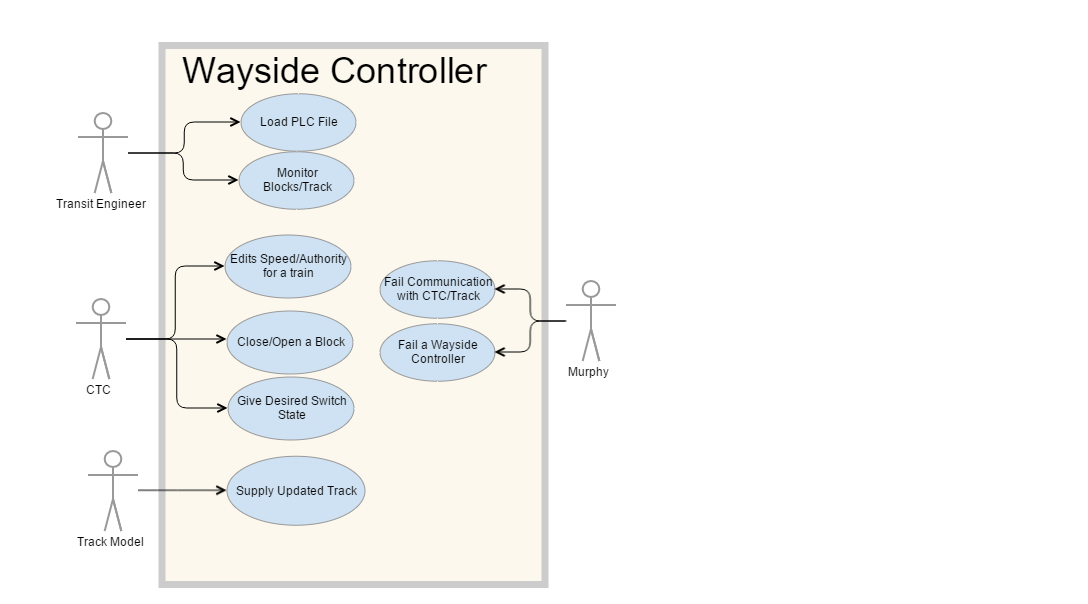
\includegraphics[scale=.3]{trackcontrollerusecase.png}
	\caption{Track controller use case diagram}
\end{figure}
\begin{table}[H]
	\centering
	\caption{Load PLC File}
	\begin{tabular}{|l|l|}
		\hline
		Actors & \parbox[t]{10cm}{Transit Engineer, Wayside Controller} \\ \hline
		Description & \parbox[t]{10cm}{A Transit Engineer will load a PLC file upon startup of the Wayside unit(s), and will do so by either browsing for a file or supplying the file path.} \\ \hline
		Data &  \parbox[t]{10cm}{PLC File's name, path} \\ \hline
		Stimulus &  \parbox[t]{10cm}{ 'Load' button pressed} \\ \hline
		Response & \parbox[t]{10cm}{Validity of File checked; Invalid File/Success of Load will be displayed to Transit Engineer}\\ \hline
		Comments & \parbox[t]{10cm}{Proper formatting/convention of PLC file is required	}  \\ \hline
	\end{tabular}
\end{table}

\begin{table}[H]
	\centering
	\caption{Monitor Blocks/Track}
	\begin{tabular}{|l|l|}
		\hline
		Actors & \parbox[t]{10cm}{Transit Engineer, Wayside Controller} \\ \hline
		Description & \parbox[t]{10cm}{For a given wayside, a Transit Engineer may select a block (by Line, Section, Block) from dropdowns to view its characteristics i.e. switch state \& crossing status (if applicable), occupancy, lights} \\ \hline
		Data &  \parbox[t]{10cm}{Track Blocks, Switches, Crossings, Lights} \\ \hline
		Stimulus &  \parbox[t]{10cm}{Block selected} \\ \hline
		Response & \parbox[t]{10cm}{Information queried from block and displayed}\\ \hline
		Comments & \parbox[t]{10cm}{Selection of blocks changes based on Wayside Controller selected}  \\ \hline
	\end{tabular}
\end{table}

\begin{table}[H]
	\centering
	\caption{Dispatch/Edit Train}
	\begin{tabular}{|l|l|}
		\hline
		Actors & \parbox[t]{10cm}{CTC, Wayside Controller} \\ \hline
		Description & \parbox[t]{10cm}{A CTC will dispatch a train/update a train with a given speed and authority (passed to wayside controller) which will then be relayed to the track model by the wayside controller.} \\ \hline
		Data &  \parbox[t]{10cm}{Speed, Authority, Block} \\ \hline
		Stimulus &  \parbox[t]{10cm}{Speed, Authority, and Block passed to Wayside Controller} \\ \hline
		Response & \parbox[t]{10cm}{Wayside sets Speed, Authority of given block on the track model}\\ \hline
		Comments & \parbox[t]{10cm}{}  \\ \hline
	\end{tabular}
\end{table}

\begin{table}[H]
	\centering
	\caption{Open/Close a Block}
	\begin{tabular}{|l|l|}
		\hline
		Actors & \parbox[t]{10cm}{CTC, Wayside Controller} \\ \hline
		Description & \parbox[t]{10cm}{The CTC will prompt the Wayside to close or open a block for maintenance.} \\ \hline
		Data &  \parbox[t]{10cm}{Block, Open/Closed Status} \\ \hline
		Stimulus &  \parbox[t]{10cm}{CTC prompts Wayside controller to close or open a block.} \\ \hline
		Response & \parbox[t]{10cm}{Wayside sets status of given Block to open/closed.}\\ \hline
		Comments & \parbox[t]{10cm}{}  \\ \hline
	\end{tabular}
\end{table}

\begin{table}[H]
	\centering
	\caption{Supply Updated Track}
	\begin{tabular}{|l|l|}
		\hline
		Actors & \parbox[t]{10cm}{Track Model, Wayside Controller} \\ \hline
		Description & \parbox[t]{10cm}{The Track Model will provide Block Occupancies, Switch statuses, and Crossing statuses to the Wayside Controller} \\ \hline
		Data &  \parbox[t]{10cm}{Block, Switch, Crossing} \\ \hline
		Stimulus &  \parbox[t]{10cm}{Track sends updated information} \\ \hline
		Response & \parbox[t]{10cm}{Wayside gives updated info to PLC code}\\ \hline
		Comments & \parbox[t]{10cm}{}  \\ \hline
	\end{tabular}
\end{table}

\begin{table}[H]
	\centering
	\caption{Fail Communication with CTC/Track Model}
	\begin{tabular}{|l|l|}
		\hline
		Actors & \parbox[t]{10cm}{Murphy, Wayside Controller} \\ \hline
		Description & \parbox[t]{10cm}{Murphy will eliminate communication between the Wayside Controller and the CTC and Track.} \\ \hline
		Data &  \parbox[t]{10cm}{N/A} \\ \hline
		Stimulus &  \parbox[t]{10cm}{ 'Communication Fail' button pressed} \\ \hline
		Response & \parbox[t]{10cm}{All Trains are stopped.}\\ \hline
		Comments & \parbox[t]{10cm}{}  \\ \hline
	\end{tabular}
\end{table}

\begin{table}[H]
	\centering
	\caption{Fail a Wayside}
	\begin{tabular}{|l|l|}
		\hline
		Actors & \parbox[t]{10cm}{Murphy, Wayside Controller} \\ \hline
		Description & \parbox[t]{10cm}{Murphy will break a Wayside Controller causing the unit to be non-responsive} \\ \hline
		Data &  \parbox[t]{10cm}{N/A} \\ \hline
		Stimulus &  \parbox[t]{10cm}{ 'Fail Wayside' button pressed} \\ \hline
		Response & \parbox[t]{10cm}{All trains within jurisdiction of Wayside's line are stopped.}\\ \hline
		Comments & \parbox[t]{10cm}{i.e. Red Line can operate if Green Line is shut down.}  \\ \hline
	\end{tabular}
\end{table}
\subsection{Train Model}
In this subsection, the use cases of the train model are provided.

\begin{figure}[H]
	\centering
	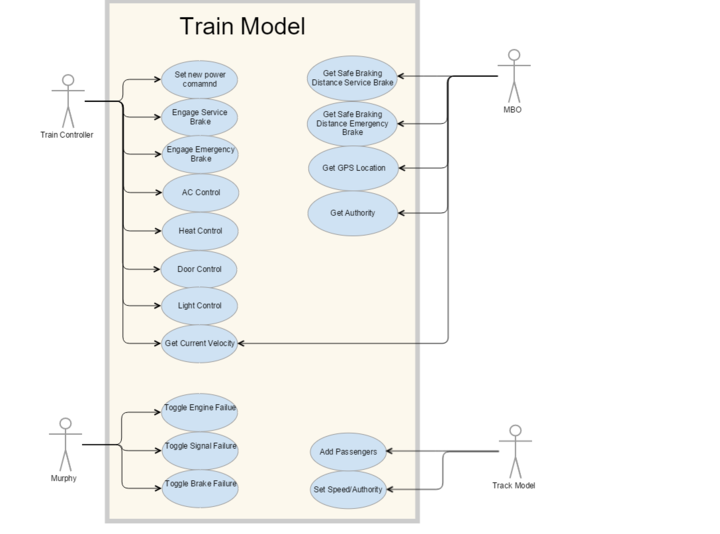
\includegraphics[scale=.3]{trainmodelusecase.png}
	\caption{Train model use case diagram}
\end{figure}
   
   \begin{table}[H]
   	\centering
   	\caption{Set New Power Command}
   	\begin{tabular}{|l|l|}
   		\hline
   		Actors & \parbox[t]{10cm}{Train Controller} \\ \hline
   		Description & \parbox[t]{10cm}{Train Controller will set a new power command based on the current velocity of the train and the new setpoint speed set by the driver. This power command will be used to determine the force applied to the train and thus compute the new current velocity.} \\ \hline
   		Data &  \parbox[t]{10cm}{Power Command issued to the train} \\ \hline
   		Stimulus &  \parbox[t]{10cm}{When a setpoint speed is provided to the train controller, a Power command is computed using the current velocity and sent to train} \\ \hline
   		Response & \parbox[t]{10cm}{New current velocity is returned to actor at the end of the computation. }\\ \hline
   		Comments & \parbox[t]{10cm}{ }  \\ \hline
   	\end{tabular}
   \end{table}
   
   \begin{table}[H]
   	\centering
   	\caption{Engage Service Brake}
   	\begin{tabular}{|l|l|}
   		\hline
   		Actors & \parbox[t]{10cm}{Train Controller} \\ \hline
   		Description & \parbox[t]{10cm}{Train controller will engage or disengage the service brake in order to slow down or stop the train for any given reason. Once engaged the power command will be set to zero and the train will begin to decelerate } \\ \hline
   		Data &  \parbox[t]{10cm}{Service Brake command } \\ \hline
   		Stimulus &  \parbox[t]{10cm}{Service brake will be engaged under the following conditions:\\1) Service brake button is manually pressed by the driver via the train controller\\2) Failure occurs in the train that requires the train to stop, this will engage the service brakes unless failure is caused by service brakes\\3) Train is set to slow down and service brakes are applied to reduce speed} \\ \hline
   		Response & \parbox[t]{10cm}{Service brake status is set to engaged and train begins to decelerate at service brake deceleration rate.}\\ \hline
   		Comments & \parbox[t]{10cm}{The service brake can either posses the status of on, off , or failure.}  \\ \hline
   	\end{tabular}
   \end{table}
   
   \begin{table}[H]
   	\centering
   	\caption{Engage Emergency Brake	}
   	\begin{tabular}{|l|l|}
   		\hline
   		Actors & \parbox[t]{10cm}{Train Controller} \\ \hline
   		Description & \parbox[t]{10cm}{Train controller will engage or disengage the emergency brake in order to slow down or stop the train for any emergencies that may occur. Once engaged the power command will be set to zero and the train will begin to decelerate } \\ \hline
   		Data &  \parbox[t]{10cm}{Emergency Brake command } \\ \hline
   		Stimulus &  \parbox[t]{10cm}{Emergency brake will be engaged under the following conditions:\\1) Emergency brake button is manually pressed by the driver or passenger via the train controller\\2) Failure occurs in the service brakes and the emergency brakes are required to stop the train  } \\ \hline
   		Response & \parbox[t]{10cm}{Emergency brake status is set to engaged and train begins to decelerate at emergency brake deceleration rate.}\\ \hline
   		Comments & \parbox[t]{10cm}{The Emergency brake can either posses the status of on or off. For this model we are assuming that the emergency brakes never fail}  \\ \hline
   	\end{tabular}
   \end{table}
   
   
   \begin{table}[H]
   	\centering
   	\caption{Air Conditioning (AC) Control}
   	\begin{tabular}{|l|l|}
   		\hline
   		Actors & \parbox[t]{10cm}{Train Controller} \\ \hline
   		Description & \parbox[t]{10cm}{Train controller will activate or deactivate the Air conditioning unit onboard the train to decrease the current temperature of the train.} \\ \hline
   		Data &  \parbox[t]{10cm}{Air conditioning command  } \\ \hline
   		Stimulus &  \parbox[t]{10cm}{The air conditioning will be turned on or off by the train controller. This will either be performed manually by the driver using a button or automatically by the train controller based on current temperature and thermostat setting.} \\ \hline
   		Response & \parbox[t]{10cm}{AC control set to on will result in a gradual decrease of the current train internal temperature. }\\ \hline
   		Comments & \parbox[t]{10cm}{The AC can either posses the status of on, off, or failure.}  \\ \hline
   	\end{tabular}
   \end{table}
   
   \begin{table}[H]
   	\centering
   	\caption{Heater Control}
   	\begin{tabular}{|l|l|}
   		\hline
   		Actors & \parbox[t]{10cm}{Train Controller} \\ \hline
   		Description & \parbox[t]{10cm}{Train controller will activate or deactivate the heating unit onboard the train to increase the current temperature of the train.} \\ \hline
   		Data &  \parbox[t]{10cm}{Heater command } \\ \hline
   		Stimulus &  \parbox[t]{10cm}{The heating unit will be turned on or off by the train controller. This will either be performed manually by the driver using a button or automatically by the train controller based on current temperature and thermostat setting.} \\ \hline
   		Response & \parbox[t]{10cm}{Heater control set to on will result in a gradual increase of the current train internal temperature. }\\ \hline
   		Comments & \parbox[t]{10cm}{The heater can either posses the status of on, off, or failure. }  \\ \hline
   	\end{tabular}
   \end{table}
   
   \begin{table}[H]
   	\centering
   	\caption{Door Control}
   	\begin{tabular}{|l|l|}
   		\hline
   		Actors & \parbox[t]{10cm}{Train Controller} \\ \hline
   		Description & \parbox[t]{10cm}{Train controller will open and close the doors on the left and right side individually using individual commands for each side. } \\ \hline
   		Data &  \parbox[t]{10cm}{Left door command, Right door command } \\ \hline
   		Stimulus &  \parbox[t]{10cm}{The left or right doors will be opened or closed by the train controller. This will either be performed manually by the driver using a button or automatically by the train controller upon arrival and departure at each station.} \\ \hline
   		Response & \parbox[t]{10cm}{If the right door command is passed, all doors on the right side are opened. If the left door command is passed, all doors on the left side are opened. }\\ \hline
   		Comments & \parbox[t]{10cm}{The Left and Right doors can either posses the status of open, closed, or failure.}  \\ \hline
   	\end{tabular}
   \end{table}
   
   \begin{table}[H]
   	\centering
   	\caption{Light Control}
   	\begin{tabular}{|l|l|}
   		\hline
   		Actors & \parbox[t]{10cm}{Train Controller} \\ \hline
   		Description & \parbox[t]{10cm}{Train controller will turn the interior lights onboard the train on and off based on time of day and location of train (e.g. within tunnel or not)} \\ \hline
   		Data &  \parbox[t]{10cm}{Interior Light command } \\ \hline
   		Stimulus &  \parbox[t]{10cm}{The lights will be toggled on and off by the train controller. This will either be performed manually by the driver using a button or automatically by the train controller based on time of day and upon entering and exiting a tunnel} \\ \hline
   		Response & \parbox[t]{10cm}{If the light command is passed, all lights onboard the train are turned on.}\\ \hline
   		Comments & \parbox[t]{10cm}{The interior lights can either posses the status of on, off, or failure. }  \\ \hline
   	\end{tabular}
   \end{table}
   
   \begin{table}[H]
   	\centering
   	\caption{Get Current Velocity}
   	\begin{tabular}{|l|l|}
   		\hline
   		Actors & \parbox[t]{10cm}{Train Controller, MBO} \\ \hline
   		Description & \parbox[t]{10cm}{A call will be made to request the current velocity of the train and this will be passed back to the actor which required it. The train controllor will request the current velocity in order to compute the power command to send to the train model. The MBO will request the current velocity in order to compute the variation between the suggested speed and the actual speed of the train.} \\ \hline
   		Data &  \parbox[t]{10cm}{Current Velocity value} \\ \hline
   		Stimulus &  \parbox[t]{10cm}{A request will be sent to the train model to obtain the current velocity of the train at that given moment} \\ \hline
   		Response & \parbox[t]{10cm}{The current velocity of the train will be returned to the caller in MPH.}\\ \hline
   		Comments & \parbox[t]{10cm}{ }  \\ \hline
   	\end{tabular}
   \end{table}
   
   \begin{table}[H]
   	\centering
   	\caption{Toggle Engine Failure}
   	\begin{tabular}{|l|l|}
   		\hline
   		Actors & \parbox[t]{10cm}{Murphy} \\ \hline
   		Description & \parbox[t]{10cm}{Murphy is able to toggle the engine failure status in order to distrupt the train's engine. Once engaged the train will be required to stop until the issue is resolved.} \\ \hline
   		Data &  \parbox[t]{10cm}{Engine Failure command} \\ \hline
   		Stimulus &  \parbox[t]{10cm}{A command will be sent to the train model from the Murphy console to toggle the failure status of the train's engine.} \\ \hline
   		Response & \parbox[t]{10cm}{The engine failure status will be toggled as a response to the command. When an engine failure occurs the service brakes are also engaged to bring the train to a stop until issues are resolved.}\\ \hline
   		Comments & \parbox[t]{10cm}{The engine failure status will toggle between failure, and non-failure. }  \\ \hline
   	\end{tabular}
   \end{table}
   
   \begin{table}[H]
   	\centering
   	\caption{Toggle Signal Failure}
   	\begin{tabular}{|l|l|}
   		\hline
   		Actors & \parbox[t]{10cm}{Murphy} \\ \hline
   		Description & \parbox[t]{10cm}{Murphy is able to toggle the signal failure status in order to distrupt the train's signaling and communication abilities. Once engaged the train will be required to stop until the issue is resolved.} \\ \hline
   		Data &  \parbox[t]{10cm}{Signal Failure command} \\ \hline
   		Stimulus &  \parbox[t]{10cm}{A command will be sent to the train model from the Murphy console to toggle the failure status of the train's signaling system.} \\ \hline
   		Response & \parbox[t]{10cm}{The signal failure status will be toggled as a response to the command. When a signal failure occurs the service brakes are also engaged to bring the train to a stop until issues are resolved.}\\ \hline
   		Comments & \parbox[t]{10cm}{The signal failure status will toggle between failure, and non-failure.}  \\ \hline
   	\end{tabular}
   \end{table}
   
   \begin{table}[H]
   	\centering
   	\caption{Toggle Brake Failure}
   	\begin{tabular}{|l|l|}
   		\hline
   		Actors & \parbox[t]{10cm}{Murphy} \\ \hline
   		Description & \parbox[t]{10cm}{Murphy is able to toggle the brake failure status in order to distrupt the train's service brake. Once engaged the train will be required to stop until the issue is resolved.} \\ \hline
   		Data &  \parbox[t]{10cm}{Brake Failure command} \\ \hline
   		Stimulus &  \parbox[t]{10cm}{A command will be sent to the train model from the Murphy console to toggle the failure status of the train's service brake} \\ \hline
   		Response & \parbox[t]{10cm}{The brake failure status will be toggled as a response to the command. When a service brake failure occurs the emergency brakes are also engaged to bring the train to a stop until issues are resolved.}\\ \hline
   		Comments & \parbox[t]{10cm}{The brake failure status will toggle between failure, and non-failure.}  \\ \hline
   	\end{tabular}
   \end{table}
   
   \begin{table}[H]
   	\centering
   	\caption{Get Safe Braking Distance (Service Brake)}
   	\begin{tabular}{|l|l|}
   		\hline
   		Actors & \parbox[t]{10cm}{MBO} \\ \hline
   		Description & \parbox[t]{10cm}{In order to better determine the train's footprint the MBO will call to obtain the safe braking distance of the Train. This will be the distance required to bring the train to a complete stop using the service brake deceleration rate. This distance will vary based on the number of passengers on board the train and the current velocity of the train.} \\ \hline
   		Data &  \parbox[t]{10cm}{Safe Braking Distance for Service Brake} \\ \hline
   		Stimulus &  \parbox[t]{10cm}{Command will be requested from the MBO to get the current safe braking distance using the service brakes which would be computed based on the current velocity and mass of the train.} \\ \hline
   		Response & \parbox[t]{10cm}{The safe braking distance using the service brakes will be returned to the MBO.}\\ \hline
   		Comments & \parbox[t]{10cm}{ }  \\ \hline
   	\end{tabular}
   \end{table}
   
   \begin{table}[H]
   	\centering
   	\caption{Get Safe Braking Distance (Emergency Brake)}
   	\begin{tabular}{|l|l|}
   		\hline
   		Actors & \parbox[t]{10cm}{MBO} \\ \hline
   		Description & \parbox[t]{10cm}{In order to better determine the train's footprint the MBO will call to obtain the safe braking distance of the Train. This will be the distance required to bring the train to a complete stop using the emergency brake deceleration rate. This distance will vary based on the number of passengers on board the train and the current velocity of the train.} \\ \hline
   		Data &  \parbox[t]{10cm}{Safe Braking Distance for Emergency Brake} \\ \hline
   		Stimulus &  \parbox[t]{10cm}{Command will be requested from the MBO to get the current safe braking distance using the emergency brakes which would be computed based on the current velocity and mass of the train.} \\ \hline
   		Response & \parbox[t]{10cm}{The safe braking distance using the emergency brakes will be returned to the MBO.}\\ \hline
   		Comments & \parbox[t]{10cm}{ }  \\ \hline
   	\end{tabular}
   \end{table}
   
   \begin{table}[H]
   	\centering
   	\caption{Get GPS Location}
   	\begin{tabular}{|l|l|}
   		\hline
   		Actors & \parbox[t]{10cm}{MBO} \\ \hline
   		Description & \parbox[t]{10cm}{The MBO will elect to receive the current GPS location to determine the train's current location to the nearest meter. This will be determined by calculating the distance traveled by the train and compute the distance into the current block to return to the MBO} \\ \hline
   		Data &  \parbox[t]{10cm}{Current Block, Distance Into block} \\ \hline
   		Stimulus &  \parbox[t]{10cm}{Command will be requested from the MBO to get the current GPS location from the train} \\ \hline
   		Response & \parbox[t]{10cm}{GPS location will be returned providing the current block the train is in as well as the distance into that current block to the nearest meter.}\\ \hline
   		Comments & \parbox[t]{10cm}{ }  \\ \hline
   	\end{tabular}
   \end{table}
   
   \begin{table}[H]
   	\centering
   	\caption{Get Authority}
   	\begin{tabular}{|l|l|}
   		\hline
   		Actors & \parbox[t]{10cm}{MBO} \\ \hline
   		Description & \parbox[t]{10cm}{The MBO will request to receive the current Authority of the given train. This will be used in conjuction with the suggested authority to determine the variation between suggested authority and actual authority for the train.} \\ \hline
   		Data &  \parbox[t]{10cm}{Current Authority} \\ \hline
   		Stimulus &  \parbox[t]{10cm}{Command will be requested from the MBO to get the current Authority from the train} \\ \hline
   		Response & \parbox[t]{10cm}{Current authority will be returned for that given train}\\ \hline
   		Comments & \parbox[t]{10cm}{ }  \\ \hline
   	\end{tabular}
   \end{table}
   
   \begin{table}[H]
   	\centering
   	\caption{Add Passengers}
   	\begin{tabular}{|l|l|}
   		\hline
   		Actors & \parbox[t]{10cm}{Track Model} \\ \hline
   		Description & \parbox[t]{10cm}{The track model will randomly generate a number of passengers to wait at a station then upon arrival to a station a random number of passengers will board based on space avaliable on the train. This number will be sent to the train model to modify passenger count and mass of train based on capacity.} \\ \hline
   		Data &  \parbox[t]{10cm}{ Number of passengers boarding} \\ \hline
   		Stimulus &  \parbox[t]{10cm}{Command will be requested from the MBO to get the current Authority from the train} \\ \hline
   		Response & \parbox[t]{10cm}{Based on space on board, a random number of passengers between 0 and amount of space will be passed to the train model}\\ \hline
   		Comments & \parbox[t]{10cm}{ }  \\ \hline
   	\end{tabular}
   \end{table}
   
   \begin{table}[H]
   	\centering
   	\caption{Set Speed/ Authority}
   	\begin{tabular}{|l|l|}
   		\hline
   		Actors & \parbox[t]{10cm}{Track Model} \\ \hline
   		Description & \parbox[t]{10cm}{The track model will pass the speed and authority to the train model. This speed and authority will then be passed to the train controller with no variation.} \\ \hline
   		Data &  \parbox[t]{10cm}{ Speed, Authority} \\ \hline
   		Stimulus &  \parbox[t]{10cm}{Command will be sent to train model with speed and authority} \\ \hline
   		Response & \parbox[t]{10cm}{Speed and authority will be passed to train controller.}\\ \hline
   		Comments & \parbox[t]{10cm}{ }  \\ \hline
   	\end{tabular}
   \end{table}
   
   \begin{table}[H]
   	\centering
   	\caption{Set Current Block}
   	\begin{tabular}{|l|l|}
   		\hline
   		Actors & \parbox[t]{10cm}{Track Model} \\ \hline
   		Description & \parbox[t]{10cm}{The track model will pass the current block the train is on as the train enters each new block area. This current block object will provide the train with the block's grade as well as its length, to be used by the train's GPS } \\ \hline
   		Data &  \parbox[t]{10cm}{Current Block} \\ \hline
   		Stimulus &  \parbox[t]{10cm}{Command will be sent to train model with current block } \\ \hline
   		Response & \parbox[t]{10cm}{Block length will be extracted for train GPS, and Block grade will be extracted for train movement calculations}\\ \hline
   		Comments & \parbox[t]{10cm}{ }  \\ \hline
   	\end{tabular}
   \end{table}

\subsection{Train Controller}
In this subsection, the use cases of the train controller are provided.

\begin{figure}[H]
	\centering
	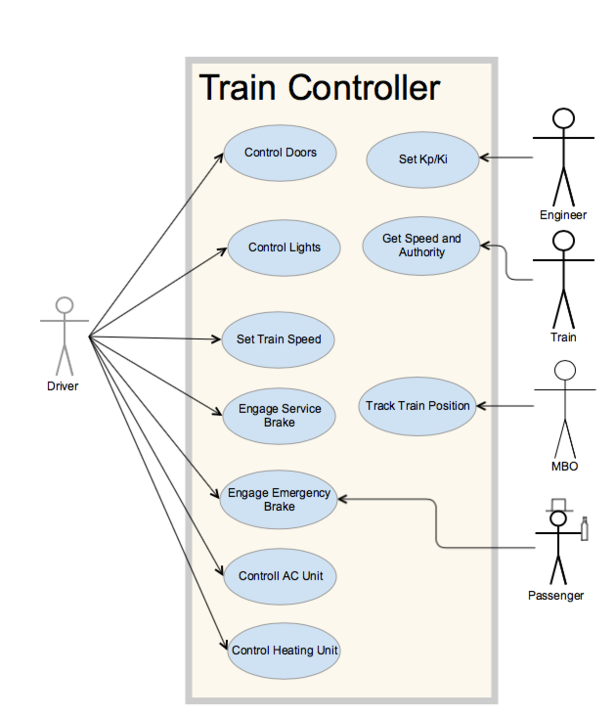
\includegraphics[scale=.2]{traincontrollerusecase.png}
	\caption{Train controller use case diagram}
\end{figure}

   \begin{table}[H]
   	\centering
   	\caption{Set Speed}
   	\begin{tabular}{|l|l|}
   		\hline
   		Actors & \parbox[t]{10cm}{Driver, Train} \\ \hline
   		Description & \parbox[t]{10cm}{Begins the process of changing the selected train's speed by using power control law. The power command is passed to the train and the train changes to a new speed.} \\ \hline
   		Data &  \parbox[t]{10cm}{Set speed, block speed, suggested speed} \\ \hline
   		Stimulus &  \parbox[t]{10cm}{'Set Speed' button is pressed or the train enters a block with a different block speed. } \\ \hline
   		Response & \parbox[t]{10cm}{Sends a power command to the selected train, signaling to either increases or decreases its speed until the actual speed equals the set speed.  }\\ \hline
   		Comments & \parbox[t]{10cm}{The set speed must not be over the suggested speed or the block speed. This is made sure by the UI elements. }  \\ \hline
   	\end{tabular}
   \end{table}
   
      \begin{table}[H]
   	\centering
   	\caption{Control Utilities}
   	\begin{tabular}{|l|l|}
   		\hline
   		Actors & \parbox[t]{10cm}{Driver, Train} \\ \hline
   		Description & \parbox[t]{10cm}{The driver will open, close, turn on, or turn off the selected train's utilities such as AC, Heat, Lights, and Left/Right Doors or the utilities will be controlled automatically by the Train Controller. } \\ \hline
   		Data &  \parbox[t]{10cm}{Selected train} \\ \hline
   		Stimulus &  \parbox[t]{10cm}{Signals transmitted from the Train Controller to the train. } \\ \hline
   		Response & \parbox[t]{10cm}{Train updates the states of the utilities. }\\ \hline
   		Comments & \parbox[t]{10cm}{AC and Heat cannot be on at the same time. }  \\ \hline
   	\end{tabular}
   \end{table}
   
      \begin{table}[H]
   	\centering
   	\caption{Set $K_{p}$ and $K_{i}$}
   	\begin{tabular}{|l|l|}
   		\hline
   		Actors & \parbox[t]{10cm}{Engineer, Train} \\ \hline
   		Description & \parbox[t]{10cm}{The engineer will set $K_p$ and $K_i$ of the selected train.} \\ \hline
   		Data &  \parbox[t]{10cm}{Train and doubles representing $K_p$ and $K_i$} \\ \hline
   		Stimulus &  \parbox[t]{10cm}{The selected train has no $K_p$ and $K_i$ set or the user clicks the 'Set $K_p$/$K_i$' button on the Train Controller.} \\ \hline
   		Response & \parbox[t]{10cm}{The $K_p$ and $K_i$ of the train will be set. }\\ \hline
   		Comments & \parbox[t]{10cm}{If the $K_p$ and the $K_i$ are not chosen for a selected train when the train is first selected, a window will pop up to allow the Engineer to set the $K_p$ and $K_i$.}  \\ \hline
   	\end{tabular}
   \end{table}

      \begin{table}[H]
   	\centering
   	\caption{Engage Service Brake}
   	\begin{tabular}{|l|l|}
   		\hline
   		Actors & \parbox[t]{10cm}{Driver, Train} \\ \hline
   		Description & \parbox[t]{10cm}{Initiates the service brake on the selected train, decreasing its speed.} \\ \hline
   		Data &  \parbox[t]{10cm}{Deceleration constant of the selected train's service brake.} \\ \hline
   		Stimulus &  \parbox[t]{10cm}{A negative power command during the power law control or user interaction.} \\ \hline
   		Response & \parbox[t]{10cm}{The service brake is engaged on the selected train, and its speed decreases.   }\\ \hline
   		Comments & \parbox[t]{10cm}{}  \\ \hline
   	\end{tabular}
   \end{table}
   
         \begin{table}[H]
   	\centering
   	\caption{Engage Emergency Brake}
   	\begin{tabular}{|l|l|}
   		\hline
   		Actors & \parbox[t]{10cm}{Driver, Train} \\ \hline
   		Description & \parbox[t]{10cm}{Initiates the emergency brake on the selected train, decreasing its speed.} \\ \hline
   		Data &  \parbox[t]{10cm}{Deceleration constant of the selected train's emergency brake.} \\ \hline
   		Stimulus &  \parbox[t]{10cm}{The emergency brake is pressed.} \\ \hline
   		Response & \parbox[t]{10cm}{The emergency brake is engaged on the selected train, and its speed decreases.  }\\ \hline
   		Comments & \parbox[t]{10cm}{In manual mode, the user must confirm the use of the emergency brake before it's actually used. }  \\ \hline
   	\end{tabular}
   \end{table}

      \begin{table}[H]
   	\centering
   	\caption{Get Speed and Authority}
   	\begin{tabular}{|l|l|}
   		\hline
   		Actors & \parbox[t]{10cm}{Train} \\ \hline
   		Description & \parbox[t]{10cm}{The Train Controller retreives the suggested speed and authority of the selected train based on which block the train is in.} \\ \hline
   		Data &  \parbox[t]{10cm}{Selected train } \\ \hline
   		Stimulus &  \parbox[t]{10cm}{During every clock tick.} \\ \hline
   		Response & \parbox[t]{10cm}{Train Controller updates its sub-components.  }\\ \hline
   		Comments & \parbox[t]{10cm}{}  \\ \hline
   	\end{tabular}
   \end{table}
   
     \begin{table}[H]
   	\centering
   	\caption{Track Train Position}
   	\begin{tabular}{|l|l|}
   		\hline
   		Actors & \parbox[t]{10cm}{MBO, Train} \\ \hline
   		Description & \parbox[t]{10cm}{Determines the position of the train on the track and sends it to the MBO when in MBO mode.} \\ \hline
   		Data &  \parbox[t]{10cm}{Block, Train} \\ \hline
   		Stimulus &  \parbox[t]{10cm}{During every clock tick.} \\ \hline
   		Response & \parbox[t]{10cm}{Train Controller updates its sub-components.  }\\ \hline
   		Comments & \parbox[t]{10cm}{}  \\ \hline
   	\end{tabular}
   \end{table}

\subsection{Moving Block Overlay}
In this subsection, the use cases of the Moving Block Overlay (MBO) are provided.

\begin{figure}[H]
	\centering
	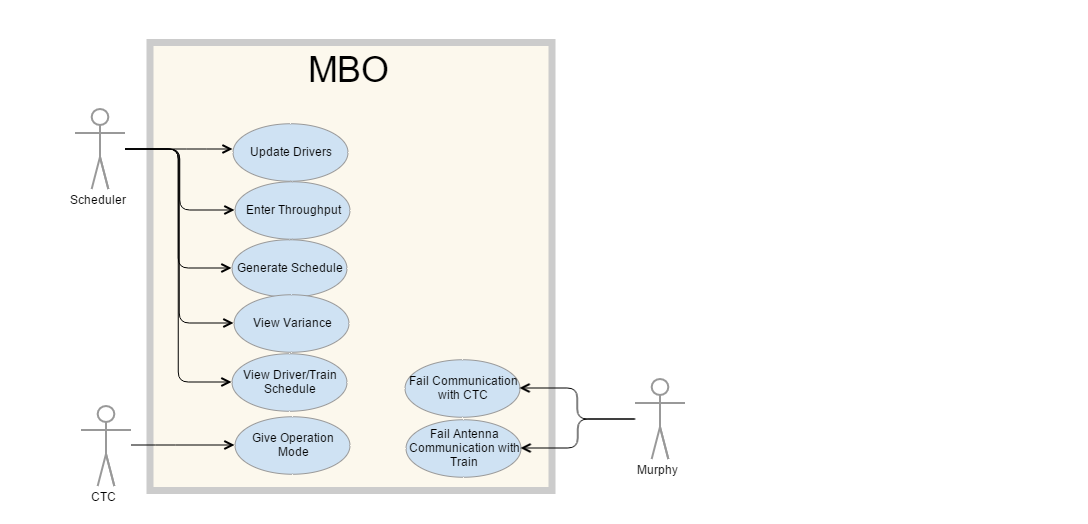
\includegraphics[scale=.2]{mbousecase.png}
	\caption{Train controller use case diagram}
\end{figure}
\begin{table}[H]
	\centering
	\caption{Update}
	\begin{tabular}{|l|l|}
		\hline
		Actors & \parbox[t]{10cm}{Scheduler} \\ \hline
		Description & \parbox[t]{10cm}{The Scheduler is able to update the list of drivers. This will change whether or not a driver is able to be scheduled.} \\ \hline
		Data &  \parbox[t]{10cm}{filename} \\ \hline
		Stimulus &  \parbox[t]{10cm}{Click drivers button} \\ \hline
		Response & \parbox[t]{10cm}{Loops through a CSV file to add all the drivers to the list of drivers. When adding a driver, a driver object will be created with the entered properties. This object will then be added to the Driver Schedule where it can be accessed as part of the list.}\\ \hline
		Comments & \parbox[t]{10cm}{There will be a default file so that it can be saved between sessions.}  \\ \hline
	\end{tabular}
\end{table}

\begin{table}[H]
	\centering
	\caption{Enter Throughput}
	\begin{tabular}{|l|l|}
		\hline
		Actors & \parbox[t]{10cm}{Scheduler} \\ \hline
		Description & \parbox[t]{10cm}{The Scheduler enters the number of trains they would like to be on the track at a certain point in time.} \\ \hline
		Data &  \parbox[t]{10cm}{number of trains} \\ \hline
		Stimulus &  \parbox[t]{10cm}{Click submit button} \\ \hline
		Response & \parbox[t]{10cm}{The number of trains is entered by the scheduler. This is used to generate both the train and driver schedules for both MBO and FB modes.}\\ \hline
		Comments & \parbox[t]{10cm}{}  \\ \hline
	\end{tabular}
\end{table}

\begin{table}[H]
	\centering
	\caption{View Train/Driver Schedule}
	\begin{tabular}{|l|l|}
		\hline
		Actors & \parbox[t]{10cm}{Scheduler, CTC} \\ \hline
		Description & \parbox[t]{10cm}{Scheduler can see a list of all  trains, as well as their station arrival times. Scheduler can see a list of all current drivers, as well as their corresponding break times and current train. } \\ \hline
		Data &  \parbox[t]{10cm}{train ID, arrival times, driver name, ID, break times} \\ \hline
		Stimulus &  \parbox[t]{10cm}{Updates triggered by clock} \\ \hline
		Response & \parbox[t]{10cm}{Two tables will be displayed, one for the train schedule, and one for the driver schedule. The train schedule will list IDs as the rows and station names as the columns. Each cell will contain the time that train will arrive at that station. The driver schedule will what train they are on at what times. It will also show whenever they start and stop work and when they are on breaks.}\\ \hline
		Comments & \parbox[t]{10cm}{The table that is displayed will automatically update itself when triggered by the clock.}  \\ \hline
	\end{tabular}
\end{table}

\begin{table}[H]
	\centering
	\caption{View Variance}
	\begin{tabular}{|l|l|}
		\hline
		Actors & \parbox[t]{10cm}{Scheduler} \\ \hline
		Description & \parbox[t]{10cm}{Scheduler can see a list of all  trains, as well as their corresponding speed and current position. The suggested speed and authority will be displayed as well as the variance between the two.} \\ \hline
		Data &  \parbox[t]{10cm}{train ID, speed, suggested/actual position/authority, variance} \\ \hline
		Stimulus &  \parbox[t]{10cm}{Updates triggered by clock} \\ \hline
		Response & \parbox[t]{10cm}{In Fixed Block mode the current block will have to be kept track of based on past block occupancy. In MBO mode the position can be gotten through GPS.}\\ \hline
		Comments & \parbox[t]{10cm}{In Fixed Block mode the position is denoted as the current block. In MBO mode the position is denoted as the current block and the distance into that block.}  \\ \hline
	\end{tabular}
\end{table}

\begin{table}[H]
	\centering
	\caption{Generate Schedules}
	\begin{tabular}{|l|l|}
		\hline
		Actors & \parbox[t]{10cm}{Scheduler} \\ \hline
		Description & \parbox[t]{10cm}{When required a schedule will be generated based on the input data. This will then be displayed for the scheduler/CTC. It is used to dispatch trains and calculate a path for a train.} \\ \hline
		Data &  \parbox[t]{10cm}{number of trains, track data} \\ \hline
		Stimulus &  \parbox[t]{10cm}{On launch, change in number of drivers, clock triggered} \\ \hline
		Response & \parbox[t]{10cm}{A schedule will be generated for trains and drivers. It will have to take into account the mode of operation (MBO or FB), speed limits, track occupancy, drivers’ break times, and other variables.}\\ \hline
		Comments & \parbox[t]{10cm}{Can only happen in automatic mode - schedule will be either fixed block or MBO depending on dispatcher's selection of mode.}  \\ \hline
	\end{tabular}
\end{table}

\begin{table}[H]
	\centering
	\caption{Give Operation Mode}
	\begin{tabular}{|l|l|}
		\hline
		Actors & \parbox[t]{10cm}{CTC} \\ \hline
		Description & \parbox[t]{10cm}{The CTC sends the mode of operation whenever it is changed.} \\ \hline
		Data &  \parbox[t]{10cm}{mode} \\ \hline
		Stimulus &  \parbox[t]{10cm}{CTC changes the mode.} \\ \hline
		Response & \parbox[t]{10cm}{The mode is updated in the MovingBlockOverlay class. Any “shutdown” procedures to switch between modes are performed.}\\ \hline
		Comments & \parbox[t]{10cm}{The default mode will be manual.}  \\ \hline
	\end{tabular}
\end{table}

\begin{table}[H]
	\centering
	\caption{Fail Communication with CTC}
	\begin{tabular}{|l|l|}
		\hline
		Actors & \parbox[t]{10cm}{Murphy} \\ \hline
		Description & \parbox[t]{10cm}{Murphy breaks communication between CTC and MBO.} \\ \hline
		Data &  \parbox[t]{10cm}{communication failure} \\ \hline
		Stimulus &  \parbox[t]{10cm}{CTC clicks Fail Communication with MBO button.} \\ \hline
		Response & \parbox[t]{10cm}{Since scheduling will be unavailable without communication with the MBO, the CTC will be forced into manual mode and let the dispatcher know with a message.}\\ \hline
		Comments & \parbox[t]{10cm}{}  \\ \hline
	\end{tabular}
\end{table}

\begin{table}[H]
	\centering
	\caption{Fail Communication with Train}
	\begin{tabular}{|l|l|}
		\hline
		Actors & \parbox[t]{10cm}{Murphy} \\ \hline
		Description & \parbox[t]{10cm}{Murphy breaks communication between Train and wayside.} \\ \hline
		Data &  \parbox[t]{10cm}{communication failure} \\ \hline
		Stimulus &  \parbox[t]{10cm}{Click Fail Communication with Train button.} \\ \hline
		Response & \parbox[t]{10cm}{The MBO can no longer receive the GPS position of individual trains and is therefore unable to safely operate in MBO mode. So a transition must be made to either Fixed Block mode or to manual mode.}\\ \hline
		Comments & \parbox[t]{10cm}{}  \\ \hline
	\end{tabular}
\end{table}

\subsection{Centralized Train Control}
In this subsection, the use cases of the Centralized Train Control (CTC) are provided.
\begin{figure}[H]
	\centering
	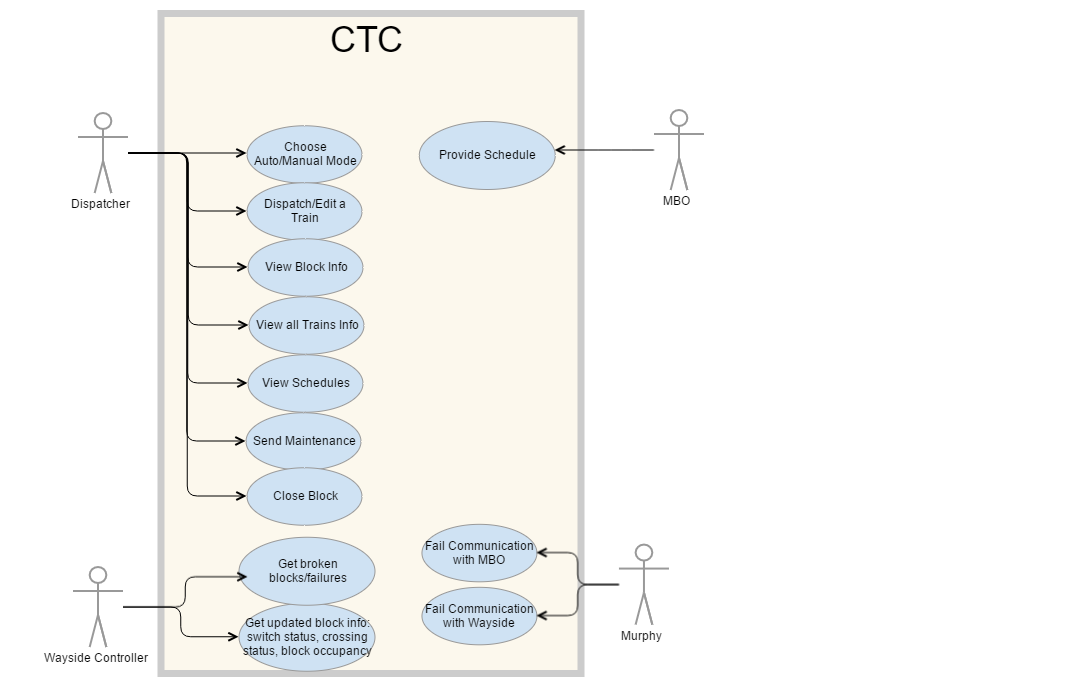
\includegraphics[scale=.15]{ctcusecase.png}
	\caption{Centralized Train Control use case}
\end{figure}

\section{Class Diagrams}
In this section, we detail the use class diagrams for each subsystem..
\subsection{Track Model}
\subsection{Track Controller}
\subsection{Train Model}
\subsection{Train Controlled}
\subsection{Moving Block Overlay}
\subsection{Centralized Train Controller}


\section{Sequence Diagrams}
In this section, we detail the sequence diagrams each subsystem.
\subsection{Track Model}
\begin{figure}[H]
	\centering
	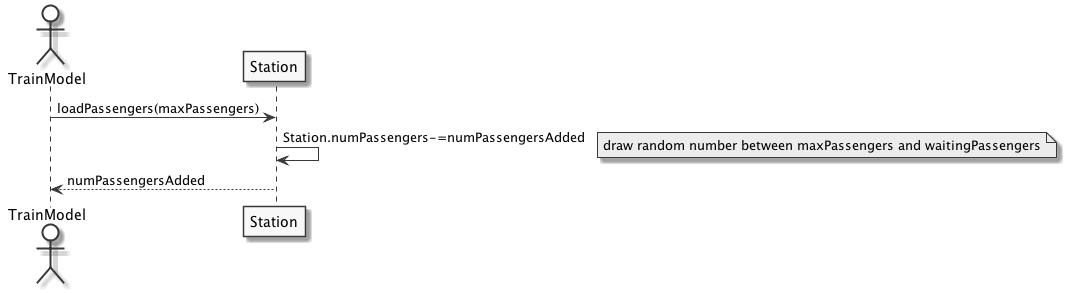
\includegraphics[scale=.3]{addPassengers.png}
	\caption{Add Passengers Use Case Diagram}
\end{figure}

\begin{figure}[H]
	\centering
	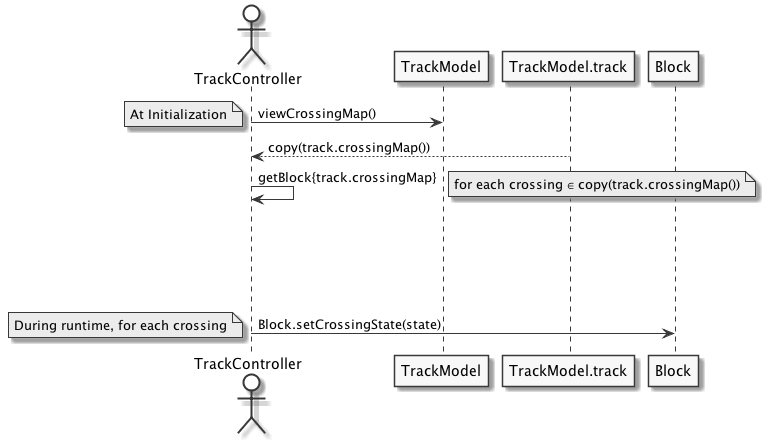
\includegraphics[scale=.3]{crossing.png}
	\caption{Toggle Crossing State Use Case Diagram}
\end{figure}

\begin{figure}[H]
	\centering
	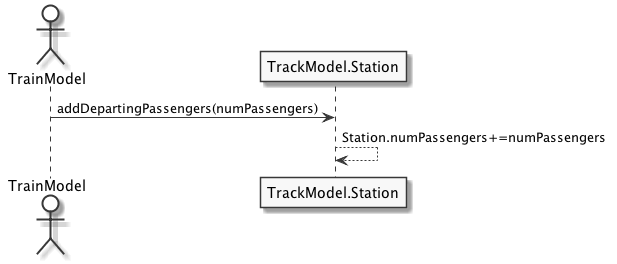
\includegraphics[scale=.3]{departPassengers.png}
	\caption{TDeparting Passengers to Station Use Case Diagram}
\end{figure}

\begin{figure}[H]
	\centering
	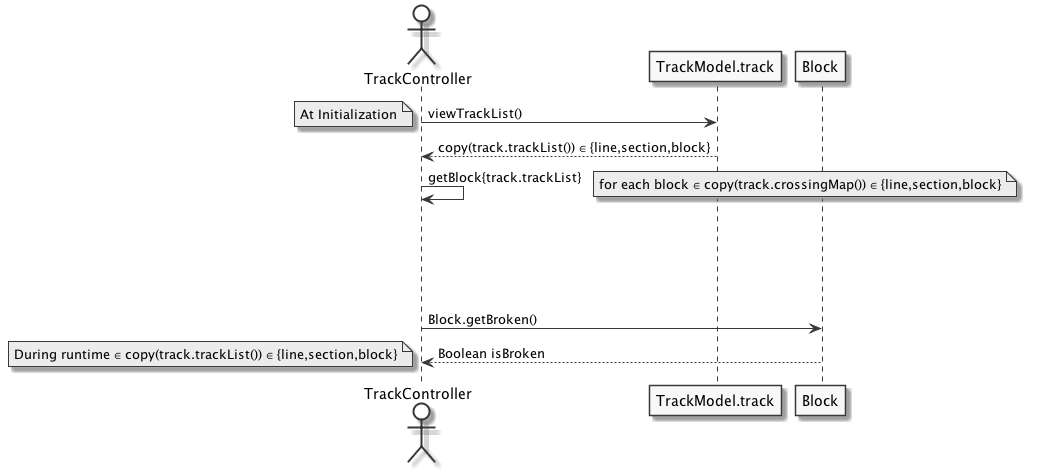
\includegraphics[scale=.3]{detectBroken.png}
	\caption{Detect Broken Rail Use Case Diagram}
\end{figure}

\begin{figure}[H]
	\centering
	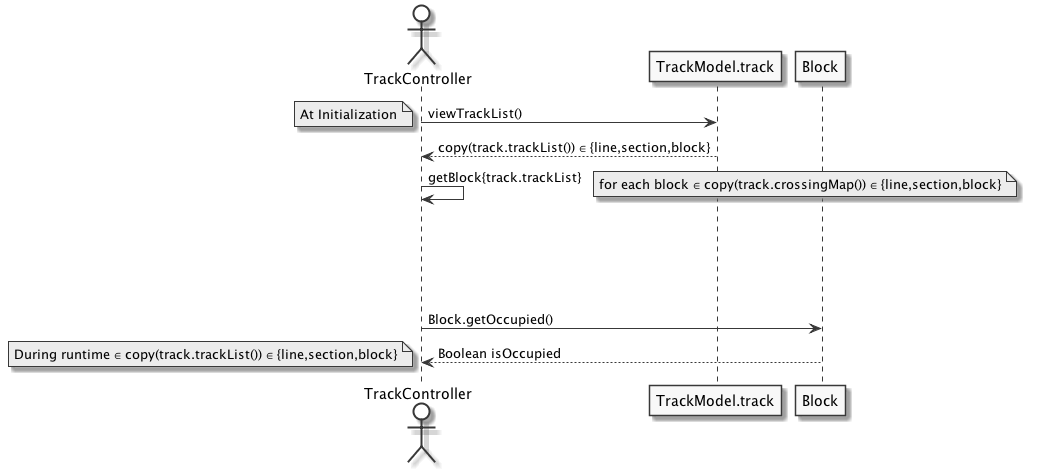
\includegraphics[scale=.3]{detectOccupied.png}
	\caption{Detect Block Occupancy use Case Diagram}
\end{figure}

\begin{figure}[H]
	\centering
	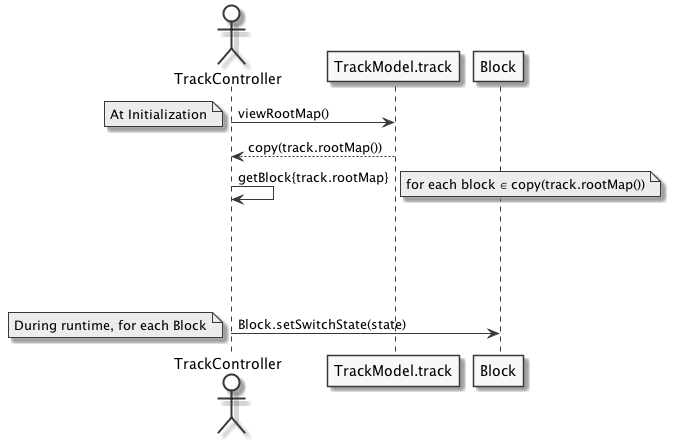
\includegraphics[scale=.3]{switching.png}
	\caption{Toggle Switching Use Case Diagram}
\end{figure}

\begin{figure}[H]
	\centering
	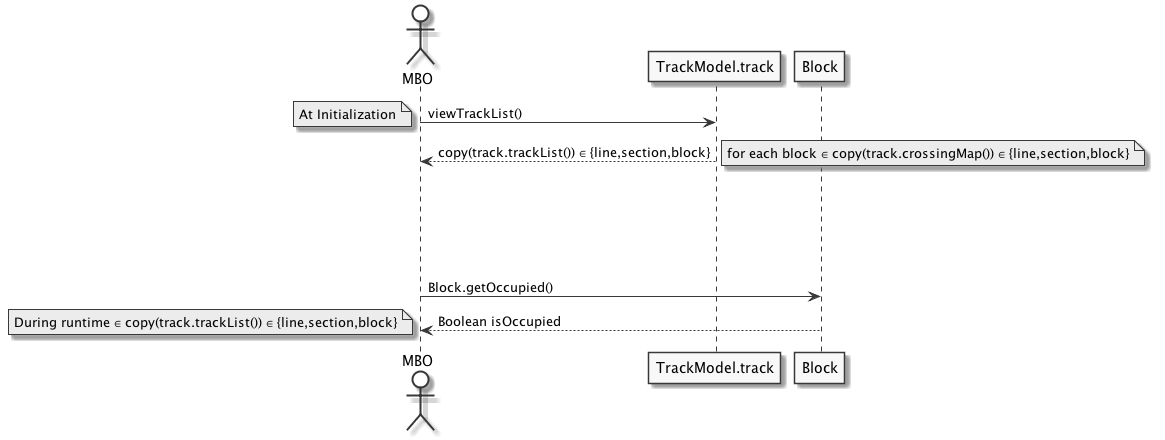
\includegraphics[scale=.3]{viewBlockOccupancy.png}
	\caption{View Block Occupancy Use Case Diagram}
\end{figure}

\begin{figure}[H]
	\centering
	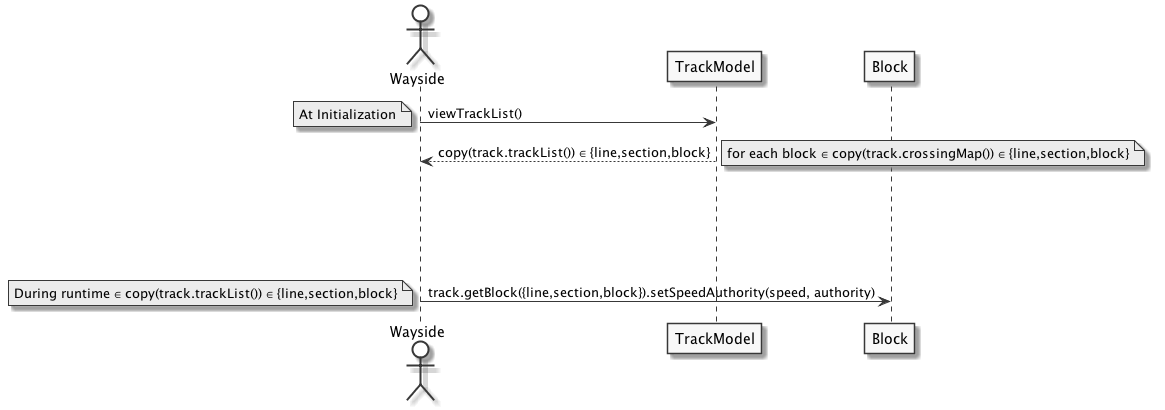
\includegraphics[scale=.3]{setSpeedAuthority.png}
	\caption{Set Speed and Authority use Case Diagram}
\end{figure}

\begin{figure}[H]
	\centering
	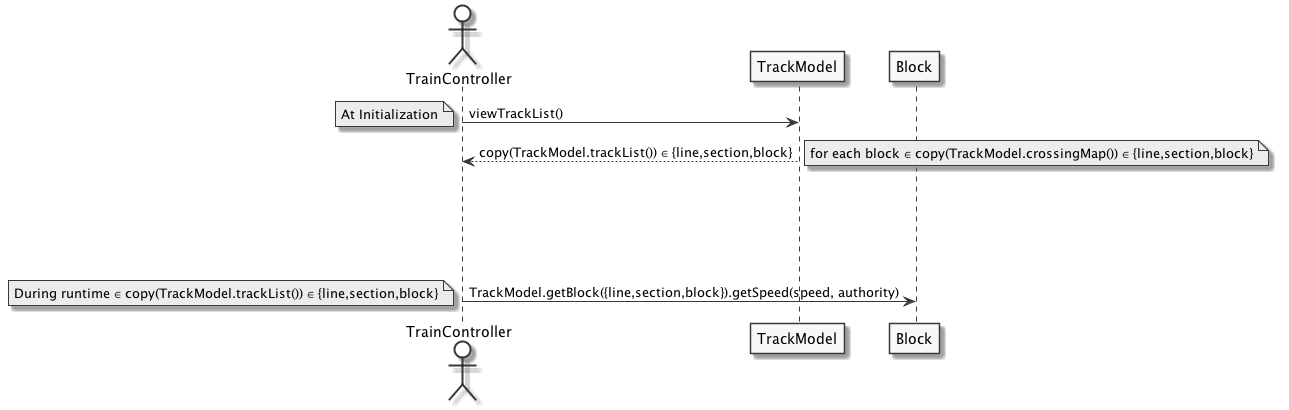
\includegraphics[scale=.3]{getSpeed.png}
	\caption{Get Speed Use Case Diagram}
\end{figure}

\begin{figure}[H]
	\centering
	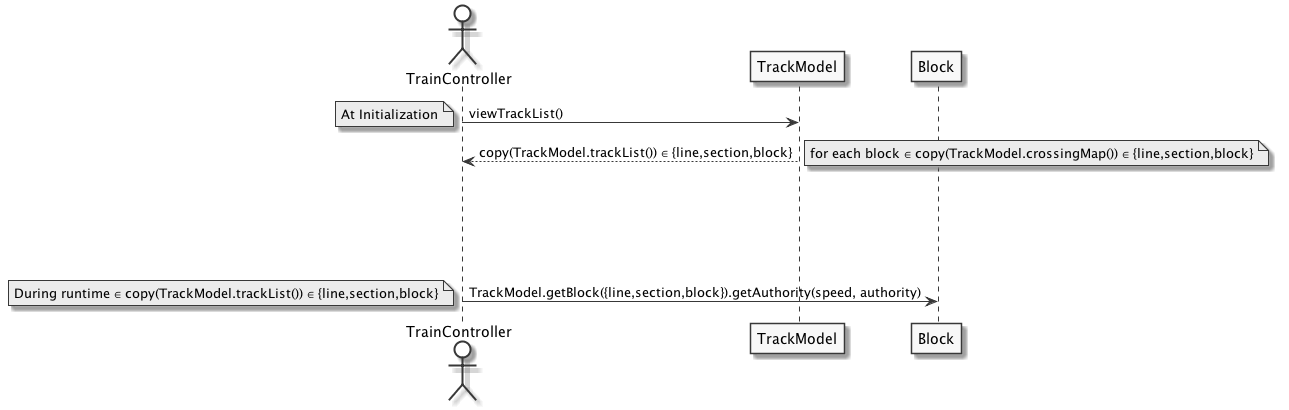
\includegraphics[scale=.3]{getAuthority.png}
	\caption{Get Authority Use Case Diagram}
\end{figure}

\begin{figure}[H]
	\centering
	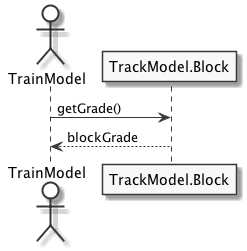
\includegraphics[scale=.3]{getGrade.png}
	\caption{Get Grade Use Case Diagram}
\end{figure}

\begin{figure}[H]
	\centering
	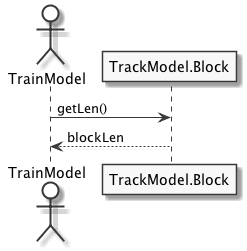
\includegraphics[scale=.3]{getLen.png}
	\caption{Get Length Use Case Diagram}
\end{figure}

\begin{figure}[H]
	\centering
	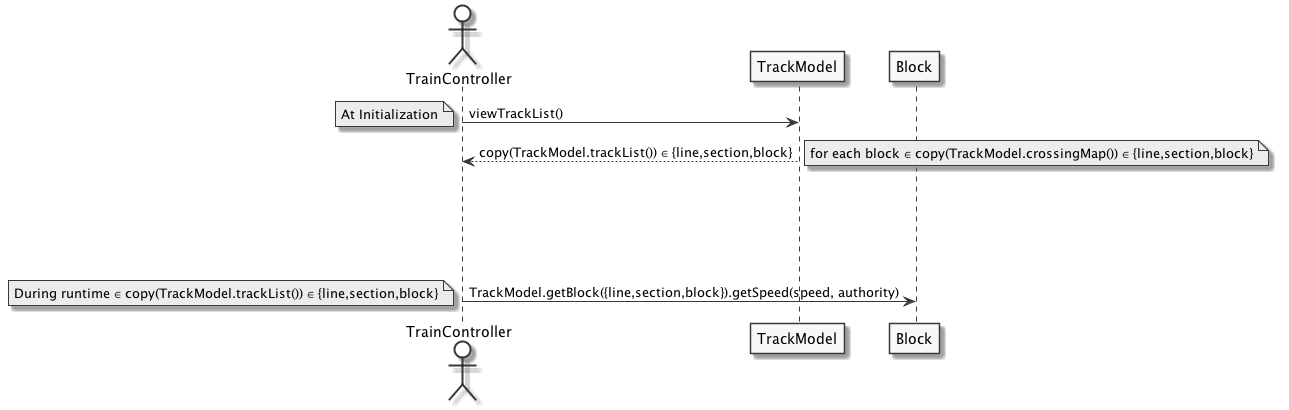
\includegraphics[scale=.3]{getSpeed.png}
	\caption{Get Speed Use Case Diagram}
\end{figure}

\begin{figure}[H]
	\centering
	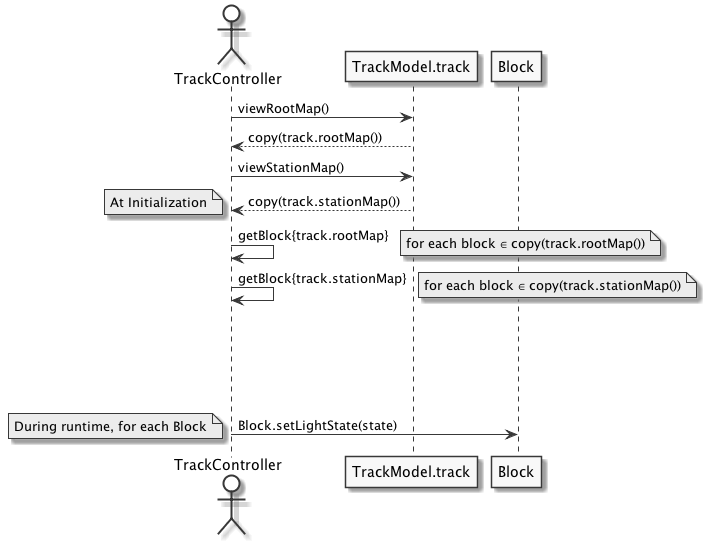
\includegraphics[scale=.3]{lights.png}
	\caption{Toggle Lights Use Case Diagram}
\end{figure}

\begin{figure}[H]
	\centering
	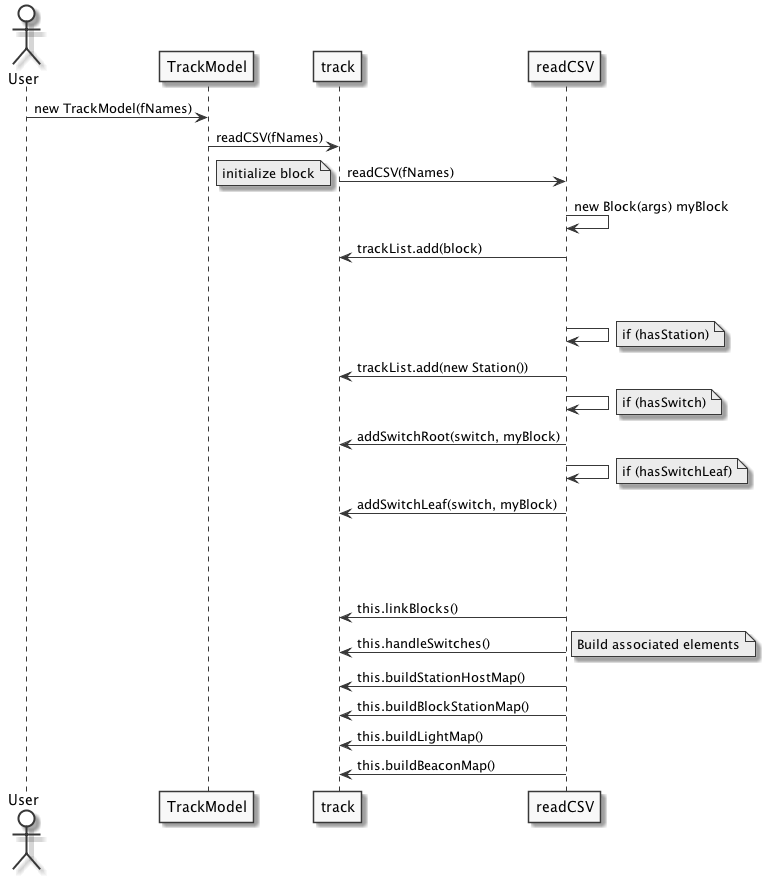
\includegraphics[scale=.3]{readFile.png}
	\caption{Read File Use Case Diagram}
\end{figure}

\subsection{Track Controller}

\subsection{Train Model}
In this seciton, we provide the sequence diagrams of the train model.
\begin{figure}[H]
	\centering
	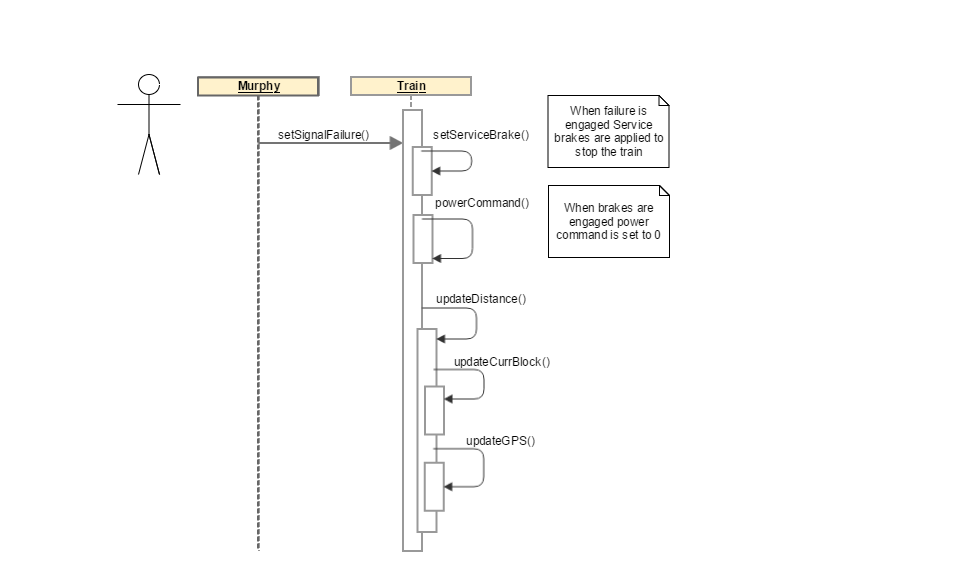
\includegraphics[scale=.3]{train_model_sqd_toggle_signal_failure.png}
	\caption{Toggle Signal Failure Use Case Diagram}
\end{figure}

\begin{figure}[H]
	\centering
	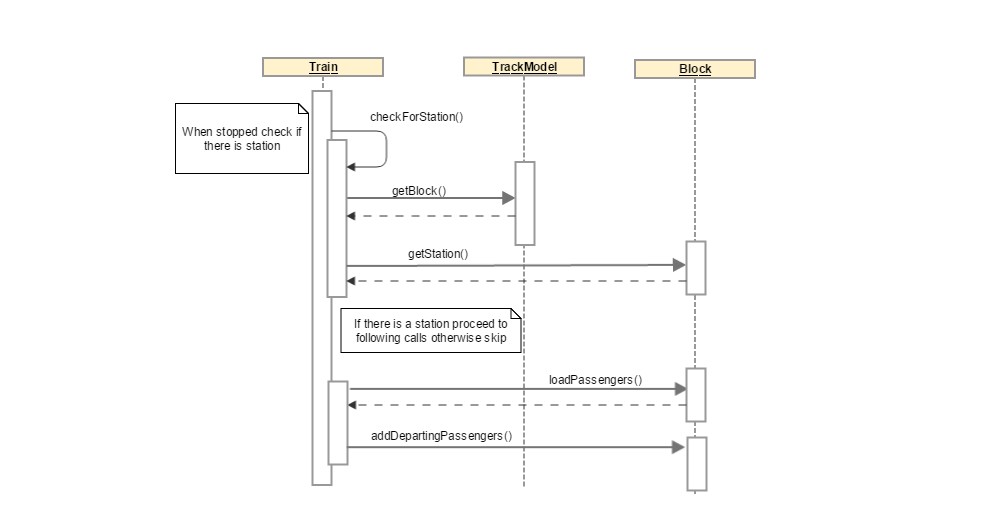
\includegraphics[scale=.3]{train_model_sqd_add_passengers.png}
	\caption{Add Passengers Use Case Diagram}
\end{figure}

\begin{figure}[H]
	\centering
	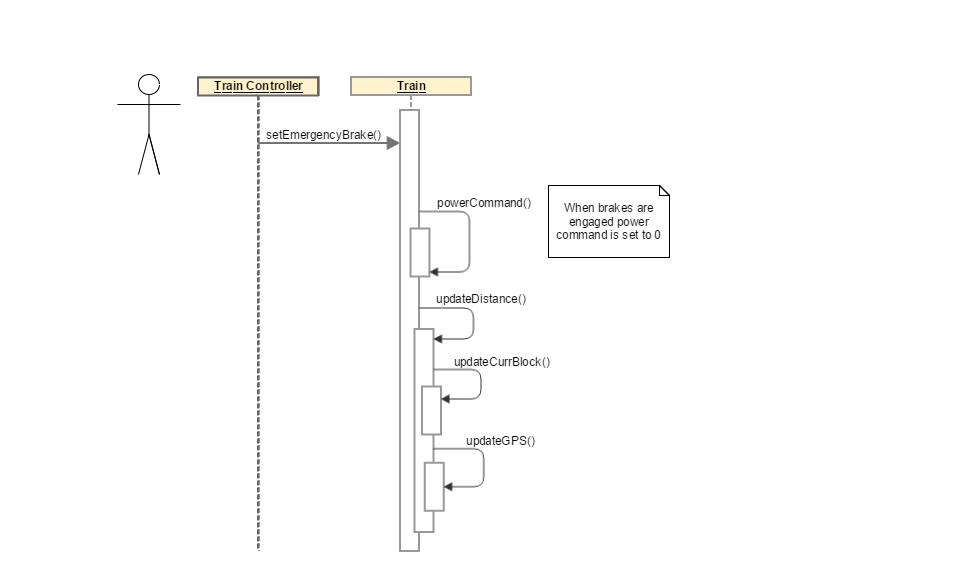
\includegraphics[scale=.3]{train_model_sqd_engage_emergency_brake.png}
	\caption{Engage Emergency Brake Use Case Diagram}
\end{figure}

\begin{figure}[H]
	\centering
	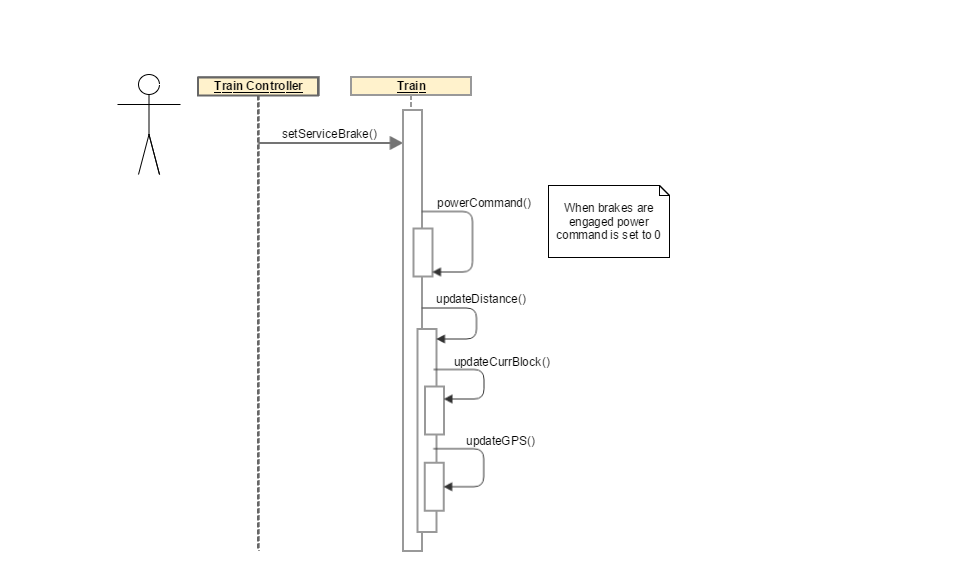
\includegraphics[scale=.3]{train_model_sqd_engage_service_brake.png}
	\caption{Engage Service Brake Use Case Diagram}
\end{figure}

\begin{figure}[H]
	\centering
	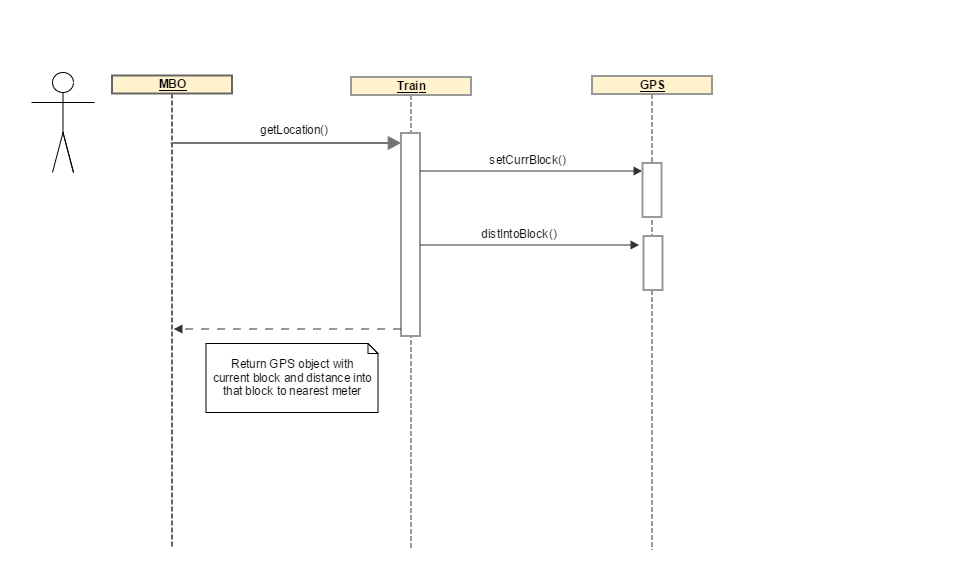
\includegraphics[scale=.3]{train_model_sqd_get_location.png}
	\caption{Get Location Use Case Diagram}
\end{figure}

\begin{figure}[H]
	\centering
	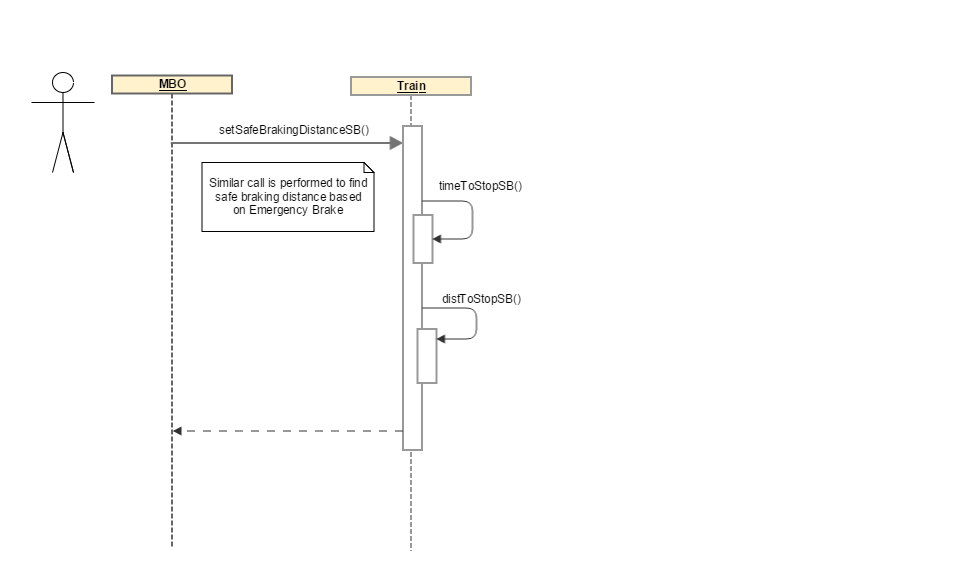
\includegraphics[scale=.3]{train_model_sqd_get_safebraking_dist.png}
	\caption{Calculate Safe Braking Distance Use Case Diagram}
\end{figure}

\begin{figure}[H]
	\centering
	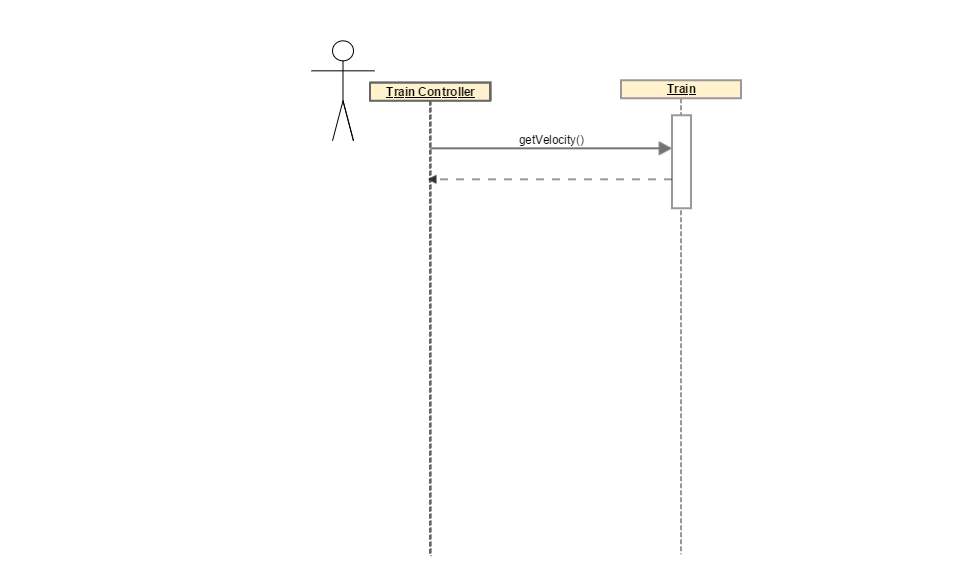
\includegraphics[scale=.3]{train_model_sqd_get_velocity.png}
	\caption{Get Velocity Use Case Diagram}
\end{figure}

\begin{figure}[H]
	\centering
	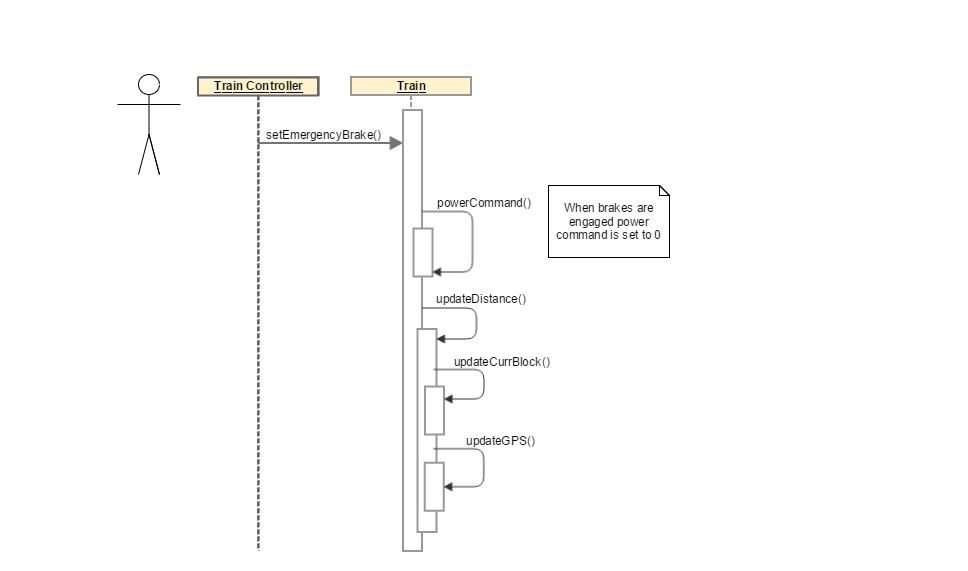
\includegraphics[scale=.3]{train_model_sqd_increase_temp.png}
	\caption{Increase Temperature Use Case Diagram}
\end{figure}

\begin{figure}[H]
	\centering
	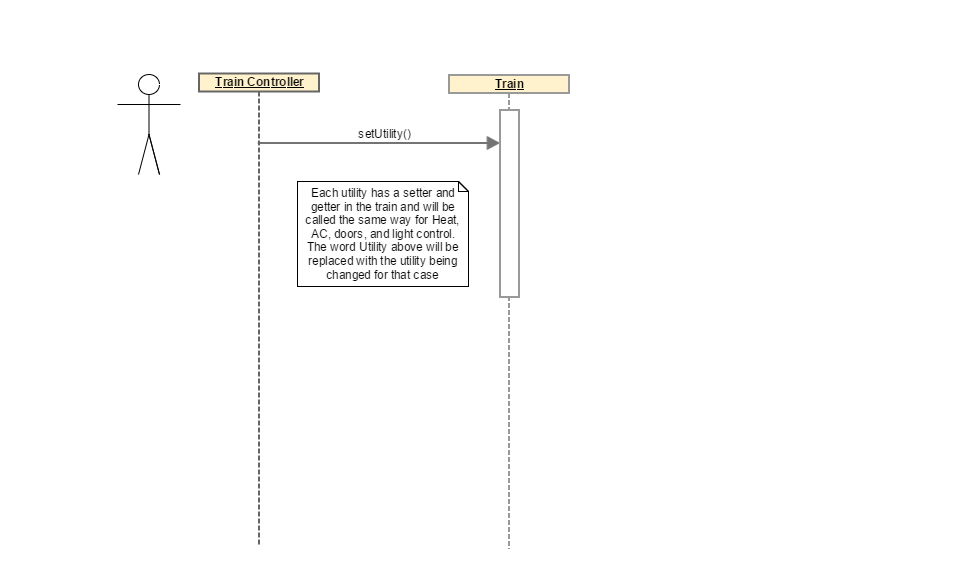
\includegraphics[scale=.3]{train_model_sqd_modify_utlilties.png}
	\caption{Modify Utilities Use Case Diagram}
\end{figure}

\begin{figure}[H]
	\centering
	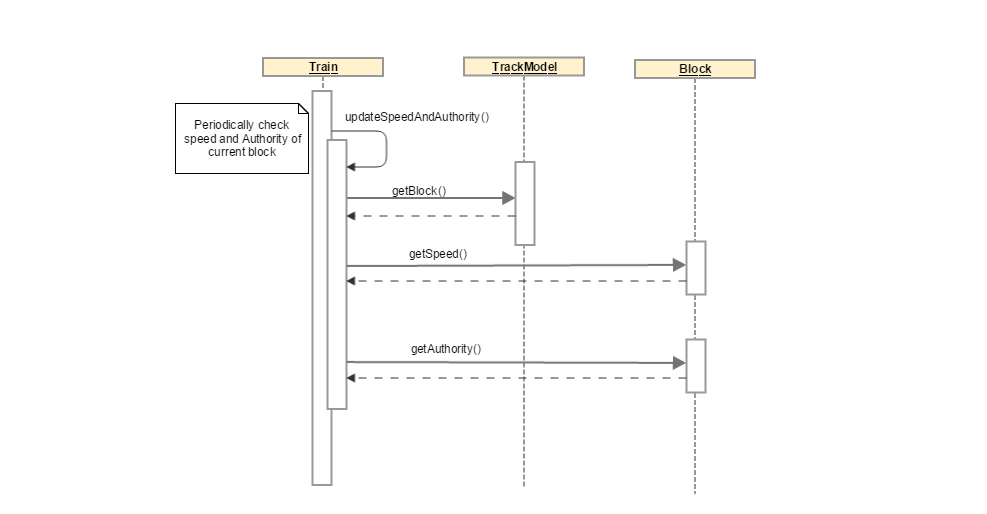
\includegraphics[scale=.3]{train_model_sqd_set_speed_authority.png}
	\caption{Set Speed and Authority Use Case Diagram}
\end{figure}

\begin{figure}[H]
	\centering
	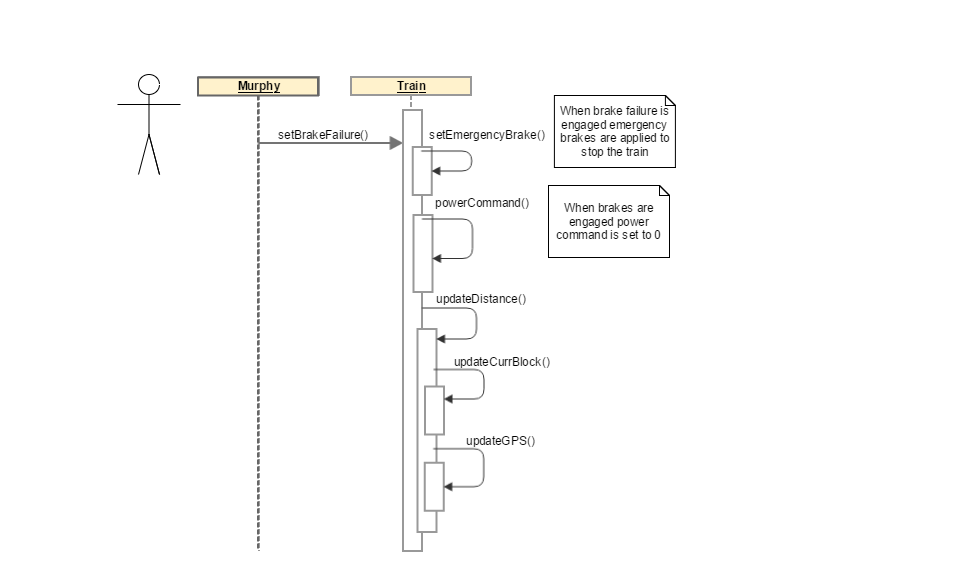
\includegraphics[scale=.3]{train_model_sqd_toggle_brake_failure.png}
	\caption{Toggle Brake Failure Use Case Diagram}
\end{figure}

\begin{figure}[H]
	\centering
	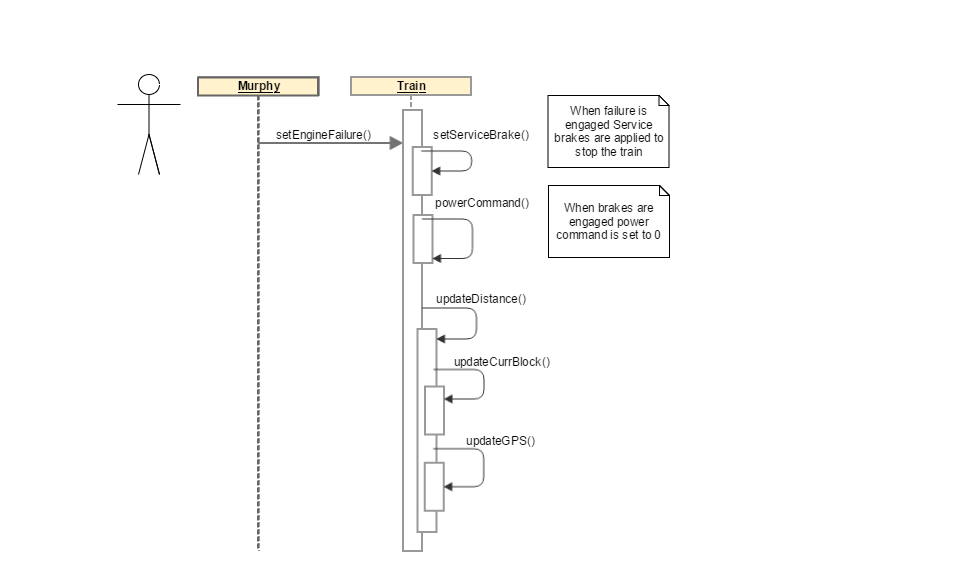
\includegraphics[scale=.3]{train_model_sqd_toggle_engine_failure.png}
	\caption{Toggle Engine Failure Use Case Diagram}
\end{figure}

\begin{figure}[H]
	\centering
	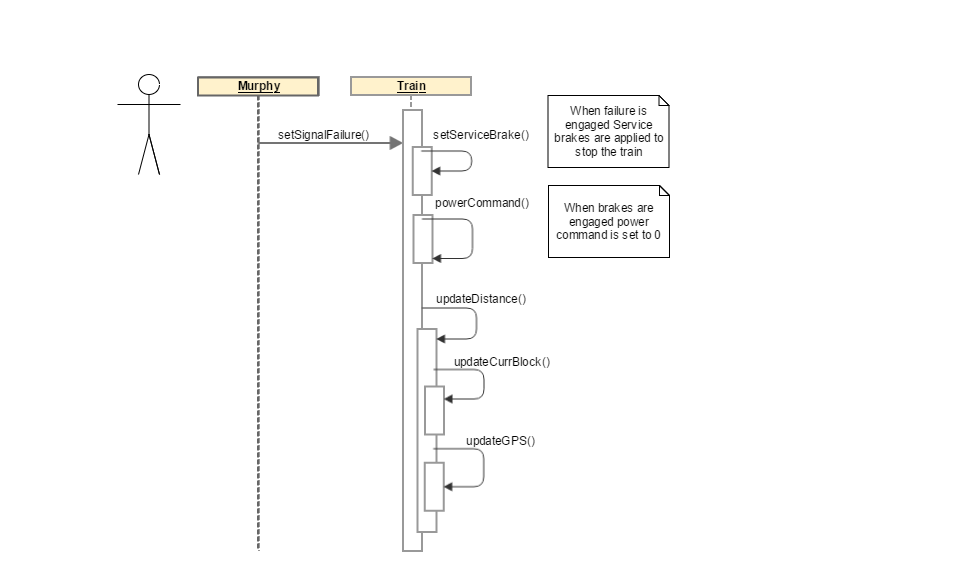
\includegraphics[scale=.3]{train_model_sqd_toggle_signal_failure.png}
	\caption{Toggle Signal Failure Use Case Diagram}
\end{figure}

\begin{figure}[H]
	\centering
	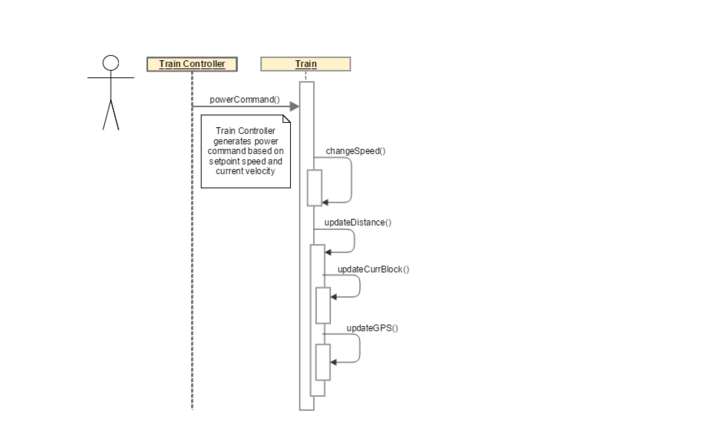
\includegraphics[scale=.3]{train_model_sqd_set_power.png}
	\caption{Toggle Signal Failure Use Case Diagram}
\end{figure}

\subsection{Train Controller}

\begin{figure}[H]
	\centering
	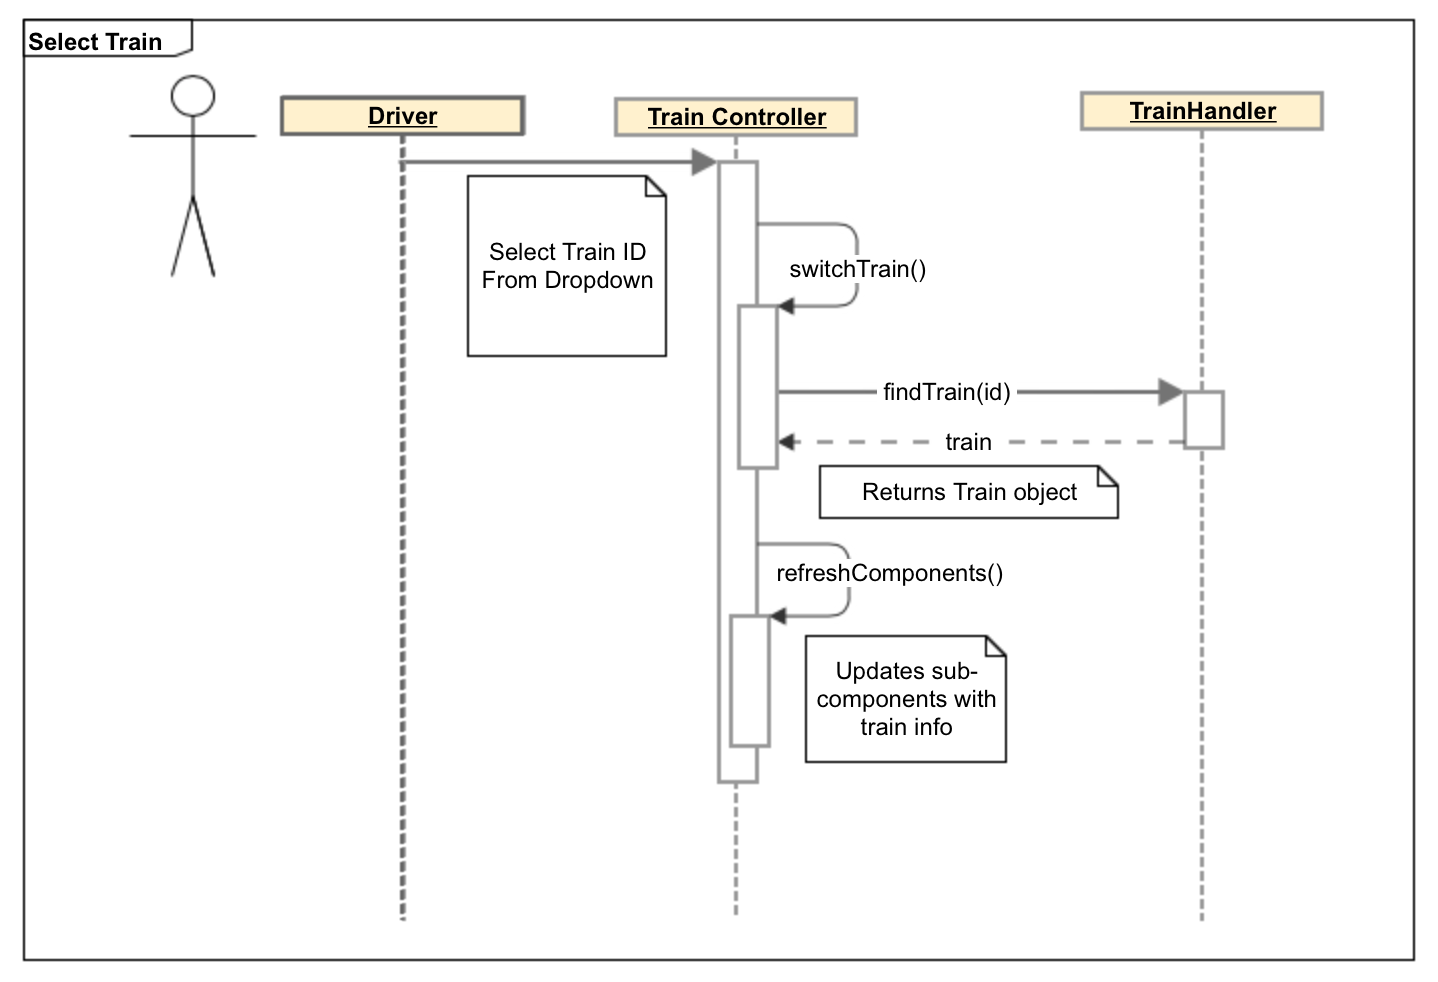
\includegraphics[scale=.3]{tc_selectTrain_usecase}
	\caption{Select Train Use Case}
\end{figure}

\begin{figure}[H]
	\centering
	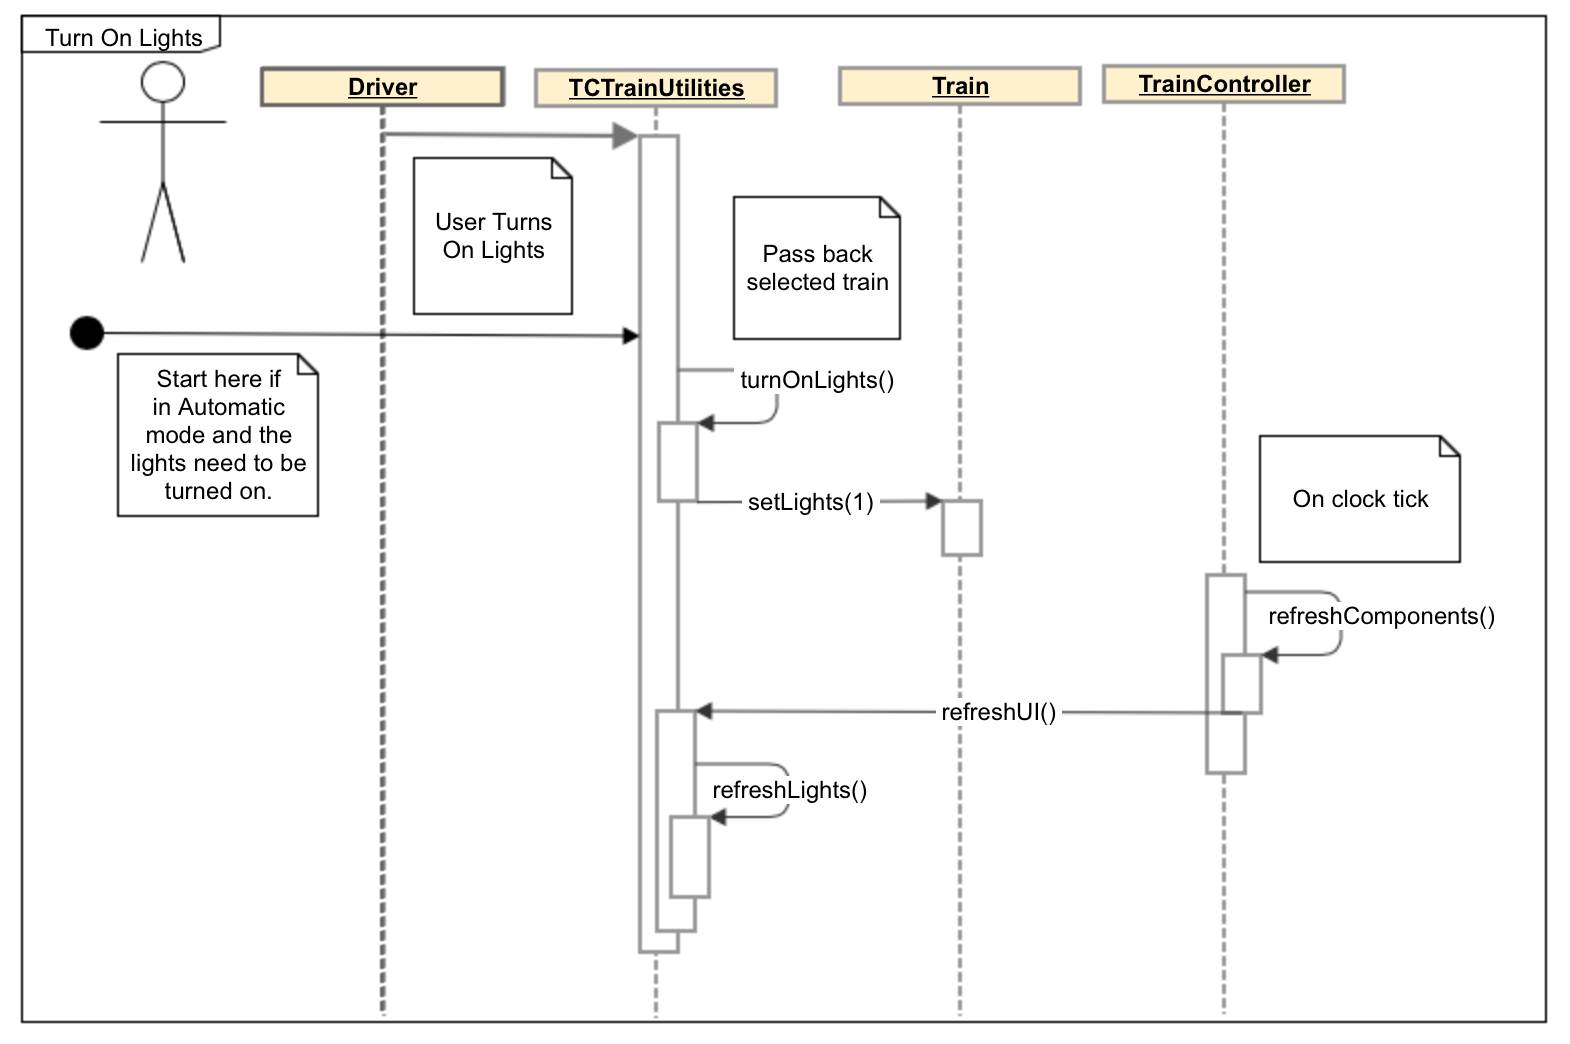
\includegraphics[scale=.3]{tc_turnOnLights_usecase}
	\caption{Turn On Lights Use Case}
\end{figure}

\begin{figure}[H]
	\centering
	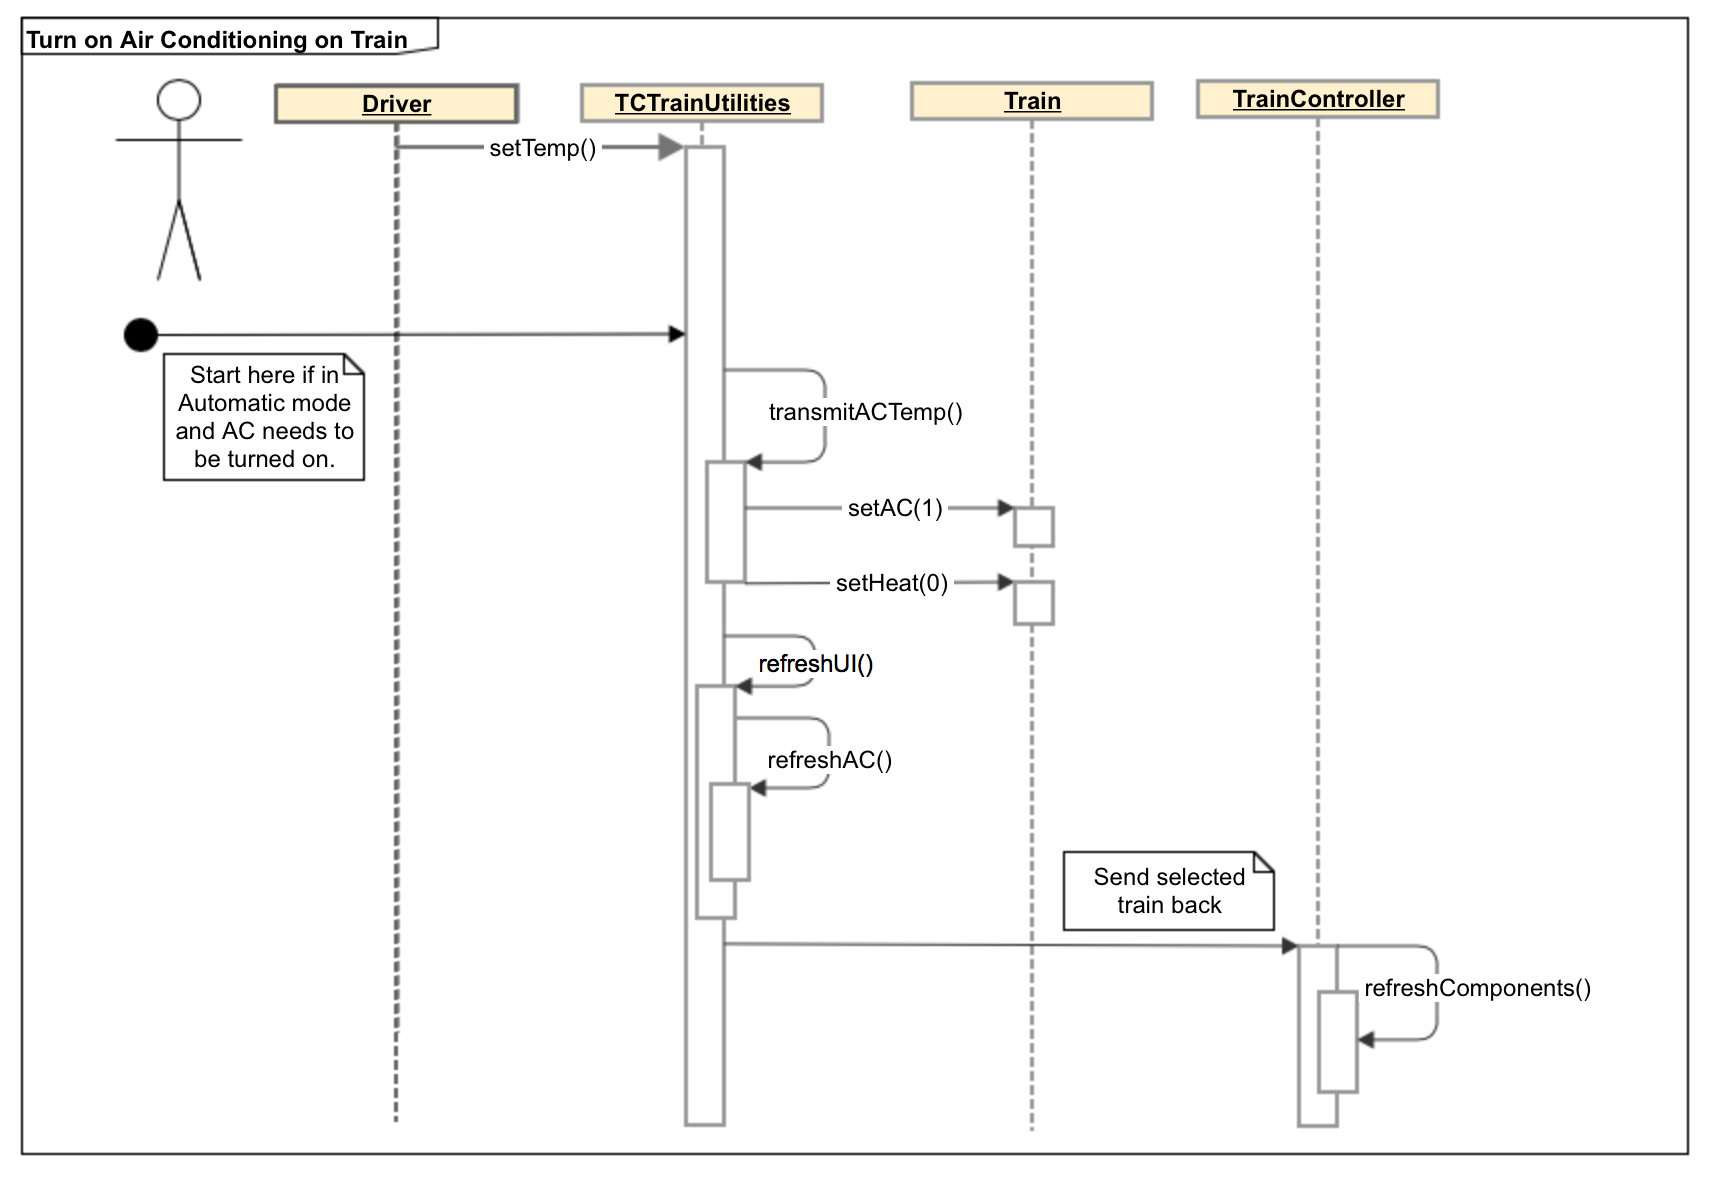
\includegraphics[scale=.3]{tc_turnOnAC_usecase}
	\caption{Turn On Air Conditioning Use Case}
\end{figure}

\begin{figure}[H]
	\centering
	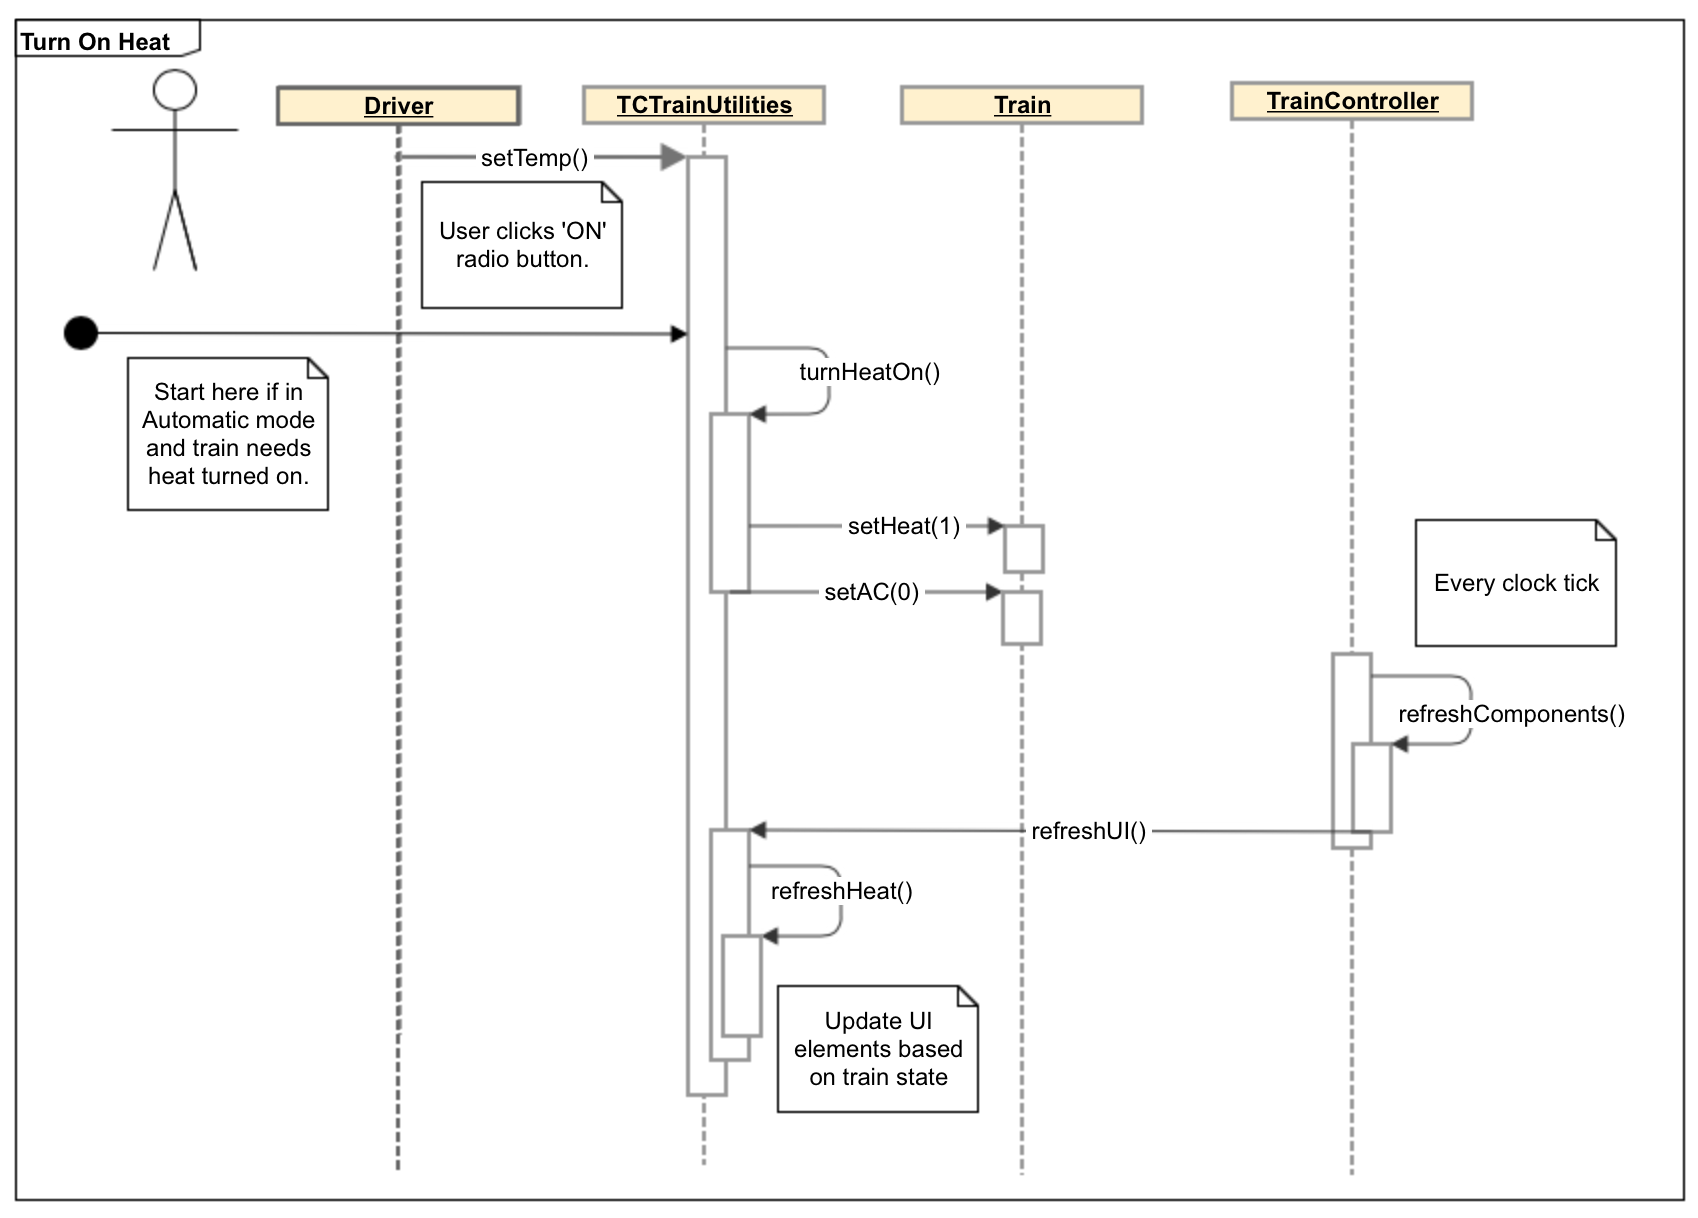
\includegraphics[scale=.3]{tc_turnOnHeat_usecase}
	\caption{Turn On Heat Use Case}
\end{figure}

\begin{figure}[H]
	\centering
	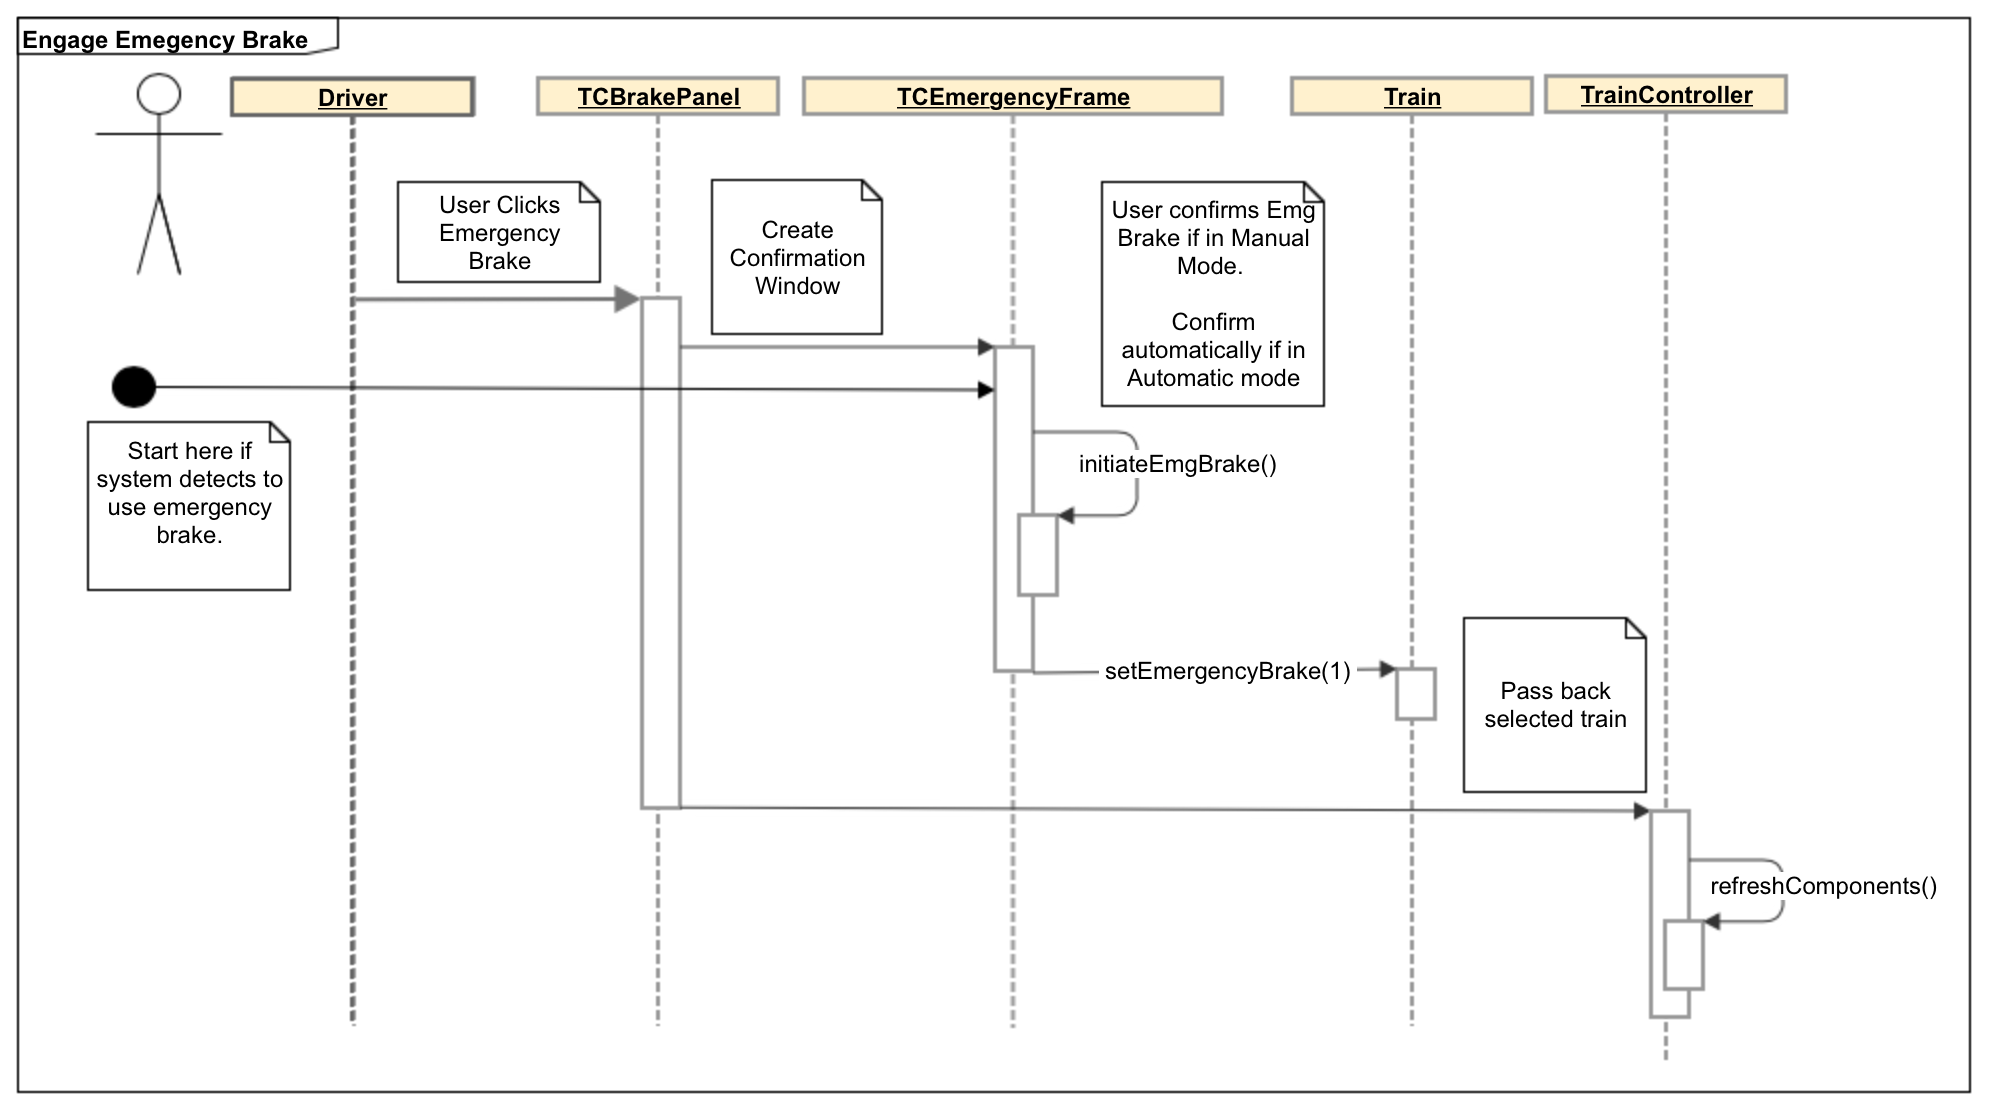
\includegraphics[scale=.3]{tc_emgBrake_usecase}
	\caption{Engage Emergency Brake Use Case}
\end{figure}

\begin{figure}[H]
	\centering
	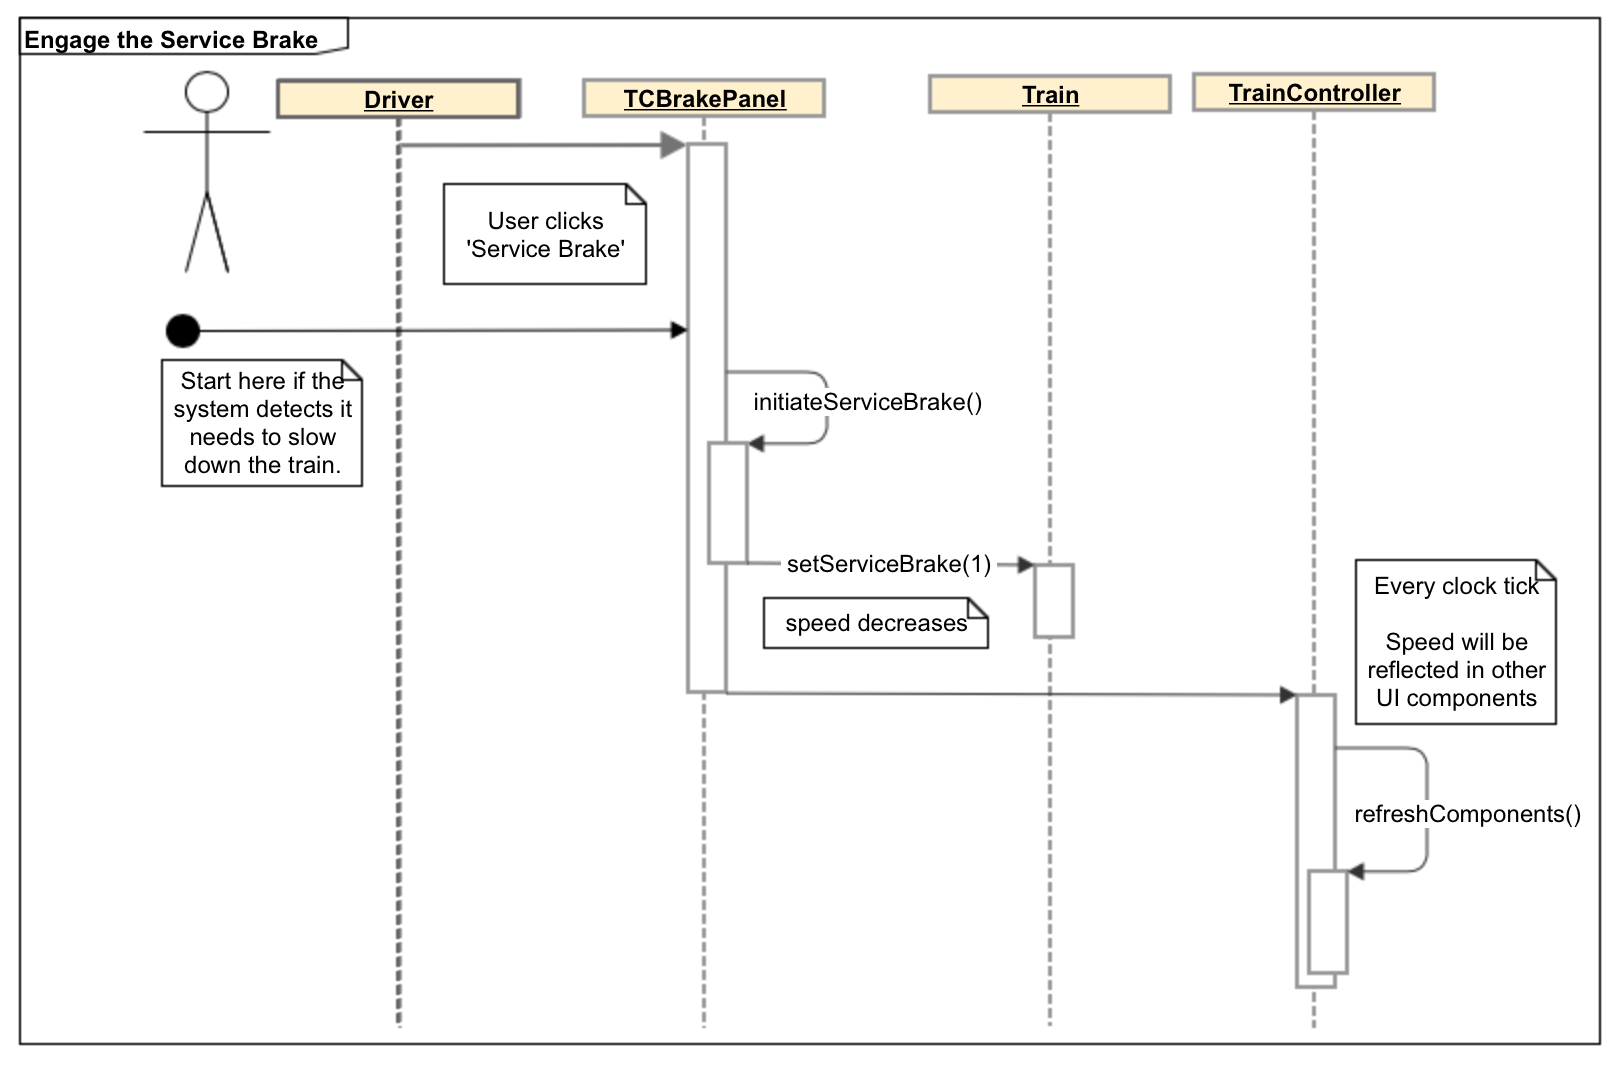
\includegraphics[scale=.3]{tc_serviceBrake_usecase}
	\caption{Engage Service Brake Use case}
\end{figure}

\begin{figure}[H]
	\centering
	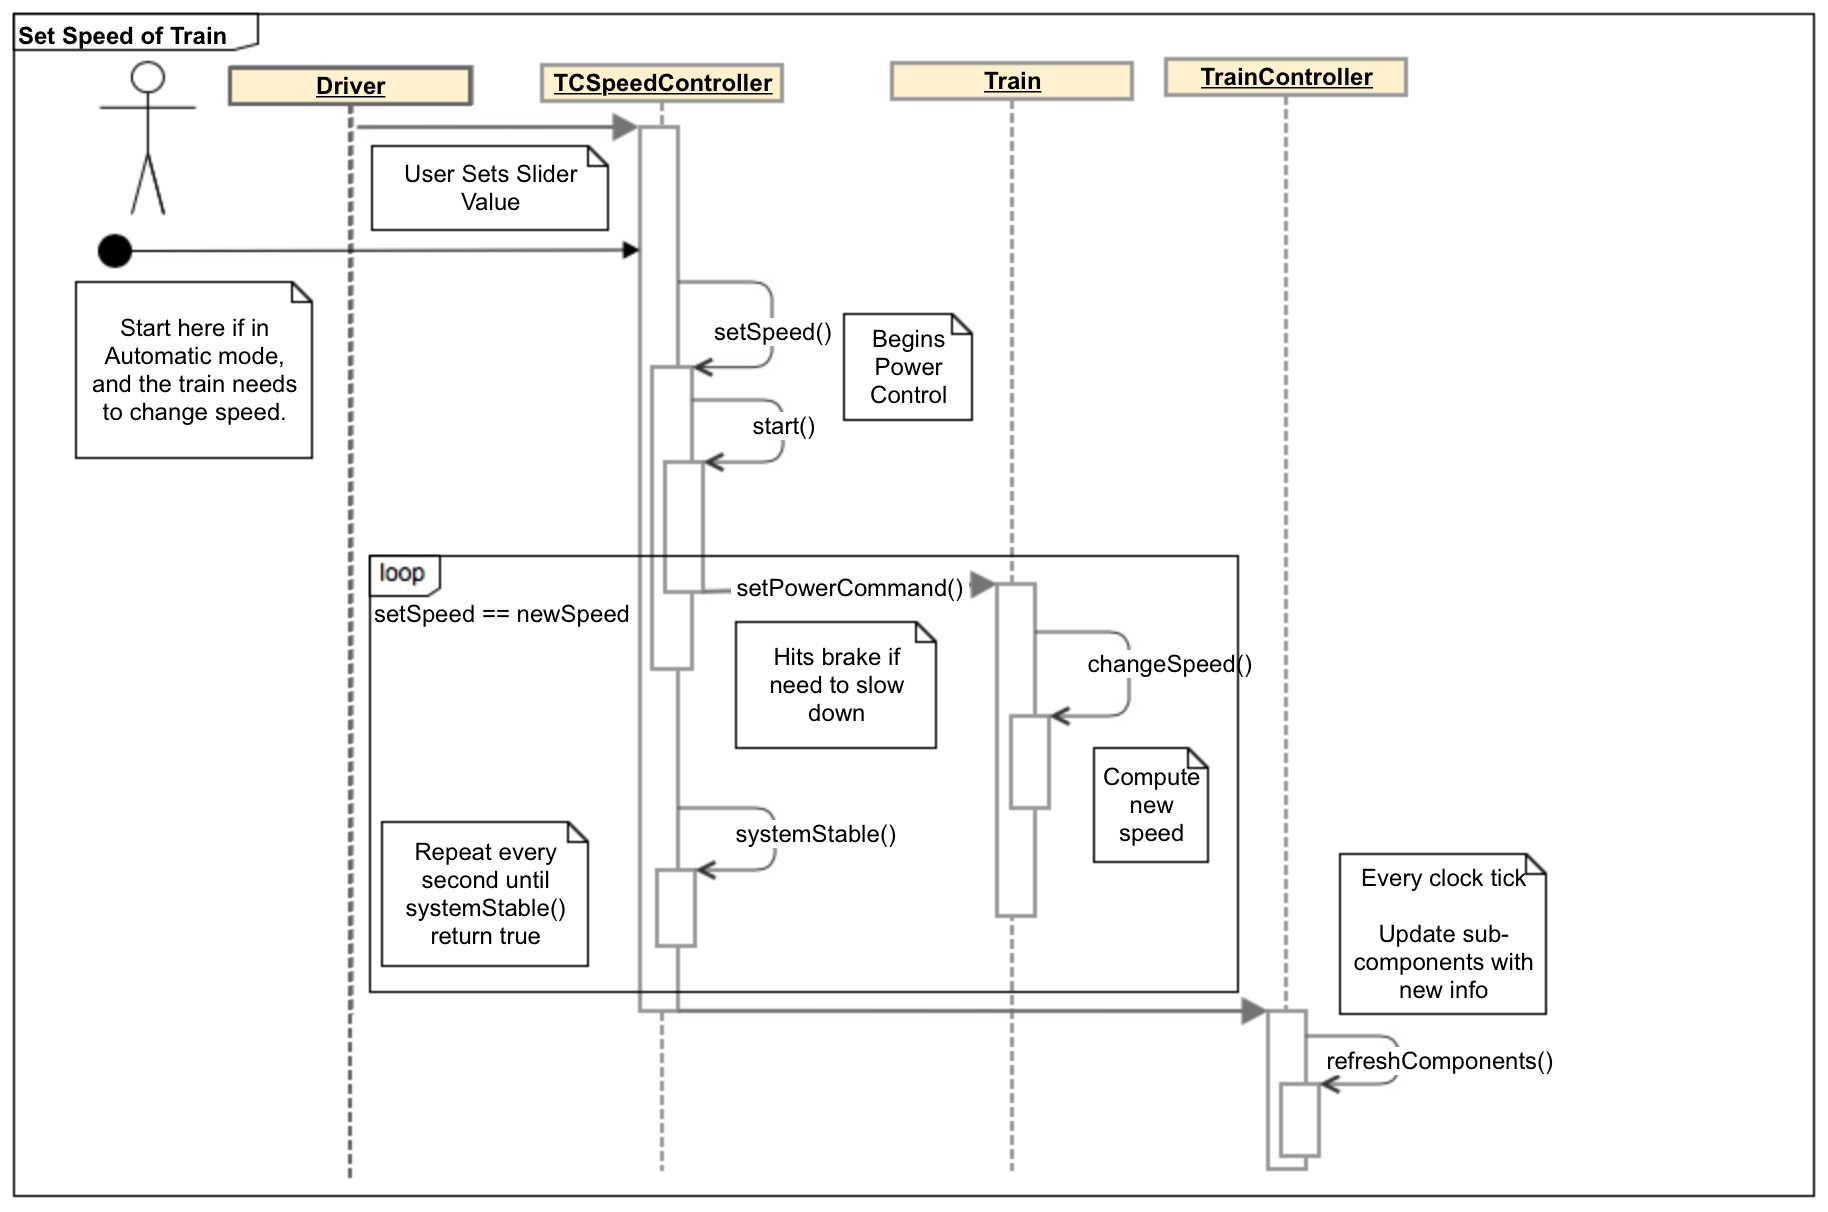
\includegraphics[scale=.3]{tc_setSpeed_usecase}
	\caption{Toggle Signal Failure Use Case Diagram}
\end{figure}



\subsection{Moving Block Overlay}
\subsection{Centralized Train Controller}


\end{document}          

